%% Modified for NDSS 2016 on 2015/10/06
%%
%% bare_conf.tex
%% V1.3
%% 2007/01/11
%% by Michael Shell
%% See:
%% http://www.michaelshell.org/
%% for current contact information.
%%
%% This is a skeleton file demonstrating the use of IEEEtran.cls
%% (requires IEEEtran.cls version 1.7 or later) with an IEEE conference paper.
%%
%% Support sites:
%% http://www.michaelshell.org/tex/ieeetran/
%% http://www.ctan.org/tex-archive/macros/latex/contrib/IEEEtran/
%% and
%% http://www.ieee.org/

%%*************************************************************************
%% Legal Notice:
%% This code is offered as-is without any warranty either expressed or
%% implied; without even the implied warranty of MERCHANTABILITY or
%% FITNESS FOR A PARTICULAR PURPOSE!
%% User assumes all risk.
%% In no event shall IEEE or any contributor to this code be liable for
%% any damages or losses, including, but not limited to, incidental,
%% consequential, or any other damages, resulting from the use or misuse
%% of any information contained here.
%%
%% All comments are the opinions of their respective authors and are not
%% necessarily endorsed by the IEEE.
%%
%% This work is distributed under the LaTeX Project Public License (LPPL)
%% ( http://www.latex-project.org/ ) version 1.3, and may be freely used,
%% distributed and modified. A copy of the LPPL, version 1.3, is included
%% in the base LaTeX documentation of all distributions of LaTeX released
%% 2003/12/01 or later.
%% Retain all contribution notices and credits.
%% ** Modified files should be clearly indicated as such, including  **
%% ** renaming them and changing author support contact information. **
%%
%% File list of work: IEEEtran.cls, IEEEtran_HOWTO.pdf, bare_adv.tex,
%%                    bare_conf.tex, bare_jrnl.tex, bare_jrnl_compsoc.tex
%%*************************************************************************

% *** Authors should verify (and, if needed, correct) their LaTeX system  ***
% *** with the testflow diagnostic prior to trusting their LaTeX platform ***
% *** with production work. IEEE's font choices can trigger bugs that do  ***
% *** not appear when using other class files.                            ***
% The testflow support page is at:
% http://www.michaelshell.org/tex/testflow/



% Note that the a4paper option is mainly intended so that authors in
% countries using A4 can easily print to A4 and see how their papers will
% look in print - the typesetting of the document will not typically be
% affected with changes in paper size (but the bottom and side margins will).
% Use the testflow package mentioned above to verify correct handling of
% both paper sizes by the user's LaTeX system.
%
% Also note that the "draftcls" or "draftclsnofoot", not "draft", option
% should be used if it is desired that the figures are to be displayed in
% draft mode.
%
\documentclass[10pt,conference]{IEEEtran}
\usepackage[pdftex,bookmarksnumbered]{hyperref}
\usepackage{amssymb}
%\setcounter{tocdepth}{3}
\usepackage{graphicx}
\usepackage{float}
\usepackage{amssymb}
\usepackage{algorithm}
\usepackage{algorithmic}
\renewcommand{\algorithmicrequire}{\textbf{Input:}}
\renewcommand{\algorithmicensure}{\textbf{Output:}}
\usepackage{subfigure}
\newcommand{\tabincell}[2]{\begin{tabular}{@{}#1@{}}#2\end{tabular}}
\usepackage{url}
\usepackage{makeidx}
\usepackage{multirow}
\usepackage{textcomp}
\usepackage{color}
\usepackage{caption}
\captionsetup{font=footnotesize}
\usepackage{pifont, footnote}

\newcommand\FIXME[1]{\textcolor{red}{FIX:}\textcolor{red}{#1}}
% Add the compsoc option for Computer Society conferences.
%
% If IEEEtran.cls has not been installed into the LaTeX system files,
% manually specify the path to it like:
% \documentclass[conference]{../sty/IEEEtran}

\pagestyle{plain}


% Some very useful LaTeX packages include:
% (uncomment the ones you want to load)


% *** MISC UTILITY PACKAGES ***
%
%\usepackage{ifpdf}
% Heiko Oberdiek's ifpdf.sty is very useful if you need conditional
% compilation based on whether the output is pdf or dvi.
% usage:
% \ifpdf
%   % pdf code
% \else
%   % dvi code
% \fi
% The latest version of ifpdf.sty can be obtained from:
% http://www.ctan.org/tex-archive/macros/latex/contrib/oberdiek/
% Also, note that IEEEtran.cls V1.7 and later provides a builtin
% \ifCLASSINFOpdf conditional that works the same way.
% When switching from latex to pdflatex and vice-versa, the compiler may
% have to be run twice to clear warning/error messages.






% *** CITATION PACKAGES ***
%
%\usepackage{cite}
% cite.sty was written by Donald Arseneau
% V1.6 and later of IEEEtran pre-defines the format of the cite.sty package
% \cite{} output to follow that of IEEE. Loading the cite package will
% result in citation numbers being automatically sorted and properly
% "compressed/ranged". e.g., [1], [9], [2], [7], [5], [6] without using
% cite.sty will become [1], [2], [5]--[7], [9] using cite.sty. cite.sty's
% \cite will automatically add leading space, if needed. Use cite.sty's
% noadjust option (cite.sty V3.8 and later) if you want to turn this off.
% cite.sty is already installed on most LaTeX systems. Be sure and use
% version 4.0 (2003-05-27) and later if using hyperref.sty. cite.sty does
% not currently provide for hyperlinked citations.
% The latest version can be obtained at:
% http://www.ctan.org/tex-archive/macros/latex/contrib/cite/
% The documentation is contained in the cite.sty file itself.






% *** GRAPHICS RELATED PACKAGES ***
%
\ifCLASSINFOpdf
  % \usepackage[pdftex]{graphicx}
  % declare the path(s) where your graphic files are
  % \graphicspath{{../pdf/}{../jpeg/}}
  % and their extensions so you won't have to specify these with
  % every instance of \includegraphics
  % \DeclareGraphicsExtensions{.pdf,.jpeg,.png}
\else
  % or other class option (dvipsone, dvipdf, if not using dvips). graphicx
  % will default to the driver specified in the system graphics.cfg if no
  % driver is specified.
  % \usepackage[dvips]{graphicx}
  % declare the path(s) where your graphic files are
  % \graphicspath{{../eps/}}
  % and their extensions so you won't have to specify these with
  % every instance of \includegraphics
  % \DeclareGraphicsExtensions{.eps}
\fi
% graphicx was written by David Carlisle and Sebastian Rahtz. It is
% required if you want graphics, photos, etc. graphicx.sty is already
% installed on most LaTeX systems. The latest version and documentation can
% be obtained at:
% http://www.ctan.org/tex-archive/macros/latex/required/graphics/
% Another good source of documentation is "Using Imported Graphics in
% LaTeX2e" by Keith Reckdahl which can be found as epslatex.ps or
% epslatex.pdf at: http://www.ctan.org/tex-archive/info/
%
% latex, and pdflatex in dvi mode, support graphics in encapsulated
% postscript (.eps) format. pdflatex in pdf mode supports graphics
% in .pdf, .jpeg, .png and .mps (metapost) formats. Users should ensure
% that all non-photo figures use a vector format (.eps, .pdf, .mps) and
% not a bitmapped formats (.jpeg, .png). IEEE frowns on bitmapped formats
% which can result in "jaggedy"/blurry rendering of lines and letters as
% well as large increases in file sizes.
%
% You can find documentation about the pdfTeX application at:
% http://www.tug.org/applications/pdftex





% *** MATH PACKAGES ***
%
%\usepackage[cmex10]{amsmath}
% A popular package from the American Mathematical Society that provides
% many useful and powerful commands for dealing with mathematics. If using
% it, be sure to load this package with the cmex10 option to ensure that
% only type 1 fonts will utilized at all point sizes. Without this option,
% it is possible that some math symbols, particularly those within
% footnotes, will be rendered in bitmap form which will result in a
% document that can not be IEEE Xplore compliant!
%
% Also, note that the amsmath package sets \interdisplaylinepenalty to 10000
% thus preventing page breaks from occurring within multiline equations. Use:
%\interdisplaylinepenalty=2500
% after loading amsmath to restore such page breaks as IEEEtran.cls normally
% does. amsmath.sty is already installed on most LaTeX systems. The latest
% version and documentation can be obtained at:
% http://www.ctan.org/tex-archive/macros/latex/required/amslatex/math/





% *** SPECIALIZED LIST PACKAGES ***
%
%\usepackage{algorithmic}
% algorithmic.sty was written by Peter Williams and Rogerio Brito.
% This package provides an algorithmic environment fo describing algorithms.
% You can use the algorithmic environment in-text or within a figure
% environment to provide for a floating algorithm. Do NOT use the algorithm
% floating environment provided by algorithm.sty (by the same authors) or
% algorithm2e.sty (by Christophe Fiorio) as IEEE does not use dedicated
% algorithm float types and packages that provide these will not provide
% correct IEEE style captions. The latest version and documentation of
% algorithmic.sty can be obtained at:
% http://www.ctan.org/tex-archive/macros/latex/contrib/algorithms/
% There is also a support site at:
% http://algorithms.berlios.de/index.html
% Also of interest may be the (relatively newer and more customizable)
% algorithmicx.sty package by Szasz Janos:
% http://www.ctan.org/tex-archive/macros/latex/contrib/algorithmicx/




% *** ALIGNMENT PACKAGES ***
%
%\usepackage{array}
% Frank Mittelbach's and David Carlisle's array.sty patches and improves
% the standard LaTeX2e array and tabular environments to provide better
% appearance and additional user controls. As the default LaTeX2e table
% generation code is lacking to the point of almost being broken with
% respect to the quality of the end results, all users are strongly
% advised to use an enhanced (at the very least that provided by array.sty)
% set of table tools. array.sty is already installed on most systems. The
% latest version and documentation can be obtained at:
% http://www.ctan.org/tex-archive/macros/latex/required/tools/


%\usepackage{mdwmath}
%\usepackage{mdwtab}
% Also highly recommended is Mark Wooding's extremely powerful MDW tools,
% especially mdwmath.sty and mdwtab.sty which are used to format equations
% and tables, respectively. The MDWtools set is already installed on most
% LaTeX systems. The lastest version and documentation is available at:
% http://www.ctan.org/tex-archive/macros/latex/contrib/mdwtools/


% IEEEtran contains the IEEEeqnarray family of commands that can be used to
% generate multiline equations as well as matrices, tables, etc., of high
% quality.


%\usepackage{eqparbox}
% Also of notable interest is Scott Pakin's eqparbox package for creating
% (automatically sized) equal width boxes - aka "natural width parboxes".
% Available at:
% http://www.ctan.org/tex-archive/macros/latex/contrib/eqparbox/





% *** SUBFIGURE PACKAGES ***
%\usepackage[tight,footnotesize]{subfigure}
% subfigure.sty was written by Steven Douglas Cochran. This package makes it
% easy to put subfigures in your figures. e.g., "Figure 1a and 1b". For IEEE
% work, it is a good idea to load it with the tight package option to reduce
% the amount of white space around the subfigures. subfigure.sty is already
% installed on most LaTeX systems. The latest version and documentation can
% be obtained at:
% http://www.ctan.org/tex-archive/obsolete/macros/latex/contrib/subfigure/
% subfigure.sty has been superceeded by subfig.sty.



%\usepackage[caption=false]{caption}
%\usepackage[font=footnotesize]{subfig}
% subfig.sty, also written by Steven Douglas Cochran, is the modern
% replacement for subfigure.sty. However, subfig.sty requires and
% automatically loads Axel Sommerfeldt's caption.sty which will override
% IEEEtran.cls handling of captions and this will result in nonIEEE style
% figure/table captions. To prevent this problem, be sure and preload
% caption.sty with its "caption=false" package option. This is will preserve
% IEEEtran.cls handing of captions. Version 1.3 (2005/06/28) and later
% (recommended due to many improvements over 1.2) of subfig.sty supports
% the caption=false option directly:
%\usepackage[caption=false,font=footnotesize]{subfig}
%
% The latest version and documentation can be obtained at:
% http://www.ctan.org/tex-archive/macros/latex/contrib/subfig/
% The latest version and documentation of caption.sty can be obtained at:
% http://www.ctan.org/tex-archive/macros/latex/contrib/caption/




% *** FLOAT PACKAGES ***
%
%\usepackage{fixltx2e}
% fixltx2e, the successor to the earlier fix2col.sty, was written by
% Frank Mittelbach and David Carlisle. This package corrects a few problems
% in the LaTeX2e kernel, the most notable of which is that in current
% LaTeX2e releases, the ordering of single and double column floats is not
% guaranteed to be preserved. Thus, an unpatched LaTeX2e can allow a
% single column figure to be placed prior to an earlier double column
% figure. The latest version and documentation can be found at:
% http://www.ctan.org/tex-archive/macros/latex/base/



%\usepackage{stfloats}
% stfloats.sty was written by Sigitas Tolusis. This package gives LaTeX2e
% the ability to do double column floats at the bottom of the page as well
% as the top. (e.g., "\begin{figure*}[!b]" is not normally possible in
% LaTeX2e). It also provides a command:
%\fnbelowfloat
% to enable the placement of footnotes below bottom floats (the standard
% LaTeX2e kernel puts them above bottom floats). This is an invasive package
% which rewrites many portions of the LaTeX2e float routines. It may not work
% with other packages that modify the LaTeX2e float routines. The latest
% version and documentation can be obtained at:
% http://www.ctan.org/tex-archive/macros/latex/contrib/sttools/
% Documentation is contained in the stfloats.sty comments as well as in the
% presfull.pdf file. Do not use the stfloats baselinefloat ability as IEEE
% does not allow \baselineskip to stretch. Authors submitting work to the
% IEEE should note that IEEE rarely uses double column equations and
% that authors should try to avoid such use. Do not be tempted to use the
% cuted.sty or midfloat.sty packages (also by Sigitas Tolusis) as IEEE does
% not format its papers in such ways.





% *** PDF, URL AND HYPERLINK PACKAGES ***
%
%\usepackage{url}
% url.sty was written by Donald Arseneau. It provides better support for
% handling and breaking URLs. url.sty is already installed on most LaTeX
% systems. The latest version can be obtained at:
% http://www.ctan.org/tex-archive/macros/latex/contrib/misc/
% Read the url.sty source comments for usage information. Basically,
% \url{my_url_here}.





% *** Do not adjust lengths that control margins, column widths, etc. ***
% *** Do not use packages that alter fonts (such as pslatex).         ***
% There should be no need to do such things with IEEEtran.cls V1.6 and later.
% (Unless specifically asked to do so by the journal or conference you plan
% to submit to, of course. )


% correct bad hyphenation here
\hyphenation{op-tical net-works semi-conduc-tor}


\begin{document}
%
% paper title
% can use linebreaks \\ within to get better formatting as desired
%\title{RandVMP: Invalidating the Analysis Knowledge about Code Virtualized Obfuscation}
\title{Protect Virtual Machine Based Code Obfuscation from Reusing Attacking Knowledge}

% author names and affiliations
% use a multiple column layout for up to three different
% affiliations
\author{%\IEEEauthorblockN{Guanghui Li, Zhanyong Tang\IEEEauthorrefmark{1}\thanks{*Corresponding author. Email address: zytang@nwu.edu.cn},...}

%\IEEEauthorblockA{School of Information Science and Technology,
%Northwest University, Xi��an, China, 710127.\\
%leegh@stumail.nwu.edu.cn, zytang@nwu.edu.cn.}

%\and
%\IEEEauthorblockN{Di Ma}
%\IEEEauthorblockA{Department of Computer and Information Science,\\
%University of Michigan-Dearborn, MI, 48128.\\
%dmadma@umich.edu.}
}

% conference papers do not typically use \thanks and this command
% is locked out in conference mode. If really needed, such as for
% the acknowledgment of grants, issue a \IEEEoverridecommandlockouts
% after \documentclass

% for over three affiliations, or if they all won't fit within the width
% of the page, use this alternative format:
%
%\author{\IEEEauthorblockN{Michael Shell\IEEEauthorrefmark{1},
%Homer Simpson\IEEEauthorrefmark{2},
%James Kirk\IEEEauthorrefmark{3},
%Montgomery Scott\IEEEauthorrefmark{3} and
%Eldon Tyrell\IEEEauthorrefmark{4}}
%\IEEEauthorblockA{\IEEEauthorrefmark{1}School of Electrical and Computer Engineering\\
%Georgia Institute of Technology,
%Atlanta, Georgia 30332--0250\\ Email: see http://www.michaelshell.org/contact.html}
%\IEEEauthorblockA{\IEEEauthorrefmark{2}Twentieth Century Fox, Springfield, USA\\
%Email: homer@thesimpsons.com}
%\IEEEauthorblockA{\IEEEauthorrefmark{3}Starfleet Academy, San Francisco, California 96678-2391\\
%Telephone: (800) 555--1212, Fax: (888) 555--1212}
%\IEEEauthorblockA{\IEEEauthorrefmark{4}Tyrell Inc., 123 Replicant Street, Los Angeles, California 90210--4321}}




% use for special paper notices
%\IEEEspecialpapernotice{(Invited Paper)}



\IEEEoverridecommandlockouts
\makeatletter\def\@IEEEpubidpullup{9\baselineskip}\makeatother
\IEEEpubid{\parbox{\columnwidth}{Permission to freely reproduce all or part
    of this paper for noncommercial purposes is granted provided that
    copies bear this notice and the full citation on the first
    page. Reproduction for commercial purposes is strictly prohibited
    without the prior written consent of the Internet Society, the
    first-named author (for reproduction of an entire paper only), and
    the author's employer if the paper was prepared within the scope
    of employment.  \\
    NDSS '17, 26 February - 1 March 2017, San Diego, CA, USA\\
    Copyright 2017 Internet Society, ISBN 1-891562-41-X\\
    http://dx.doi.org/10.14722/ndss.2017.23xxx
}
\hspace{\columnsep}\makebox[\columnwidth]{}}


% make the title area
\maketitle



\begin{abstract}
%\boldmath
Code virtualization built upon virtual machine (VM)
technologies are emerging as a viable method for implementing
code obfuscation to protect programs against unauthorized
analysis.
State-of-the-art VM-based protection approaches use a fixed set of virtual
instructions and bytecode interpreters across programs. This allows an
experienced attacker to use knowledge extracted from other programs to
quickly attack applications protected under the same code obfuscation scheme.
In this paper, we propose a novel VM-code obfuscation system to address the
issue of reusing attacking knowledge. We achieve this by employing the
instruction set randomization technique to obfuscate the relationship between
the opcodes of bytecode instructions and their semantics. Our approach
partitions the protected code region to multiple segments where each segment
will be randomized in a different way. As a result, the same opcode of a
bytecode instruction can be mapped to different semantics in different parts
of the obfuscated code. We evaluate our approach on \FIXME{xx} real-world
applications and compare it against state-of-the-art VM-based code
obfuscation approaches. Experimental results show that our approach provides
stronger protection at the cost of little extra overhead.


%Code virtualized obfuscation, aka VM (Virtual Machine)-based obfuscation, obfuscates a software program by transforming its native instructions into bytecode instructions for a self-defined virtual instruction set architecture. The execution instruction semantics of the original program are fulfilled by a custom virtual interpreter bundled with the bytecode. Code virtualized obfuscation has been widely used by malware writers and benign software vendors to protect their programs from unauthorized analyses.
%
%The general idea of reverse analyzing a VM-obfuscated program is through extracting the program's original logic from the interpretation of the bytecode instructions, which is time-consuming and error-prone. Unfortunately, the analysis process could proceed more efficiently if the analyst is aware of the semantics of each bytecode instructions from previously obtained \textit{analysis knowledge}. To obscure the semantics of bytecode instructions, we adopt the idea of ISR (Instruction Set Randomization) to randomize the relationship between the \textit{opcodes} of bytecode instructions and their semantics. Furthermore, we partition the whole bytecode program into several parts, each part with a distinct randomization. As a result, an opcode probably means different semantics in different parts of the bytecode program. We implement a POC prototype named DCVP and conduct some experiments to evaluate the spatial and temporal overhead of DCVP. The experimental results demonstrate that DCVP is both effective and practical for obscuring the semantics of bytecode instructions, and thus for hindering unauthorized analyses.
\end{abstract}


% no keywords
\begin{IEEEkeywords}
Virtualized obfuscation, reverse engineering, instruction set randomization, analysis knowledge
\end{IEEEkeywords}



% For peer review papers, you can put extra information on the cover
% page as needed:
% \ifCLASSOPTIONpeerreview
% \begin{center} \bfseries EDICS Category: 3-BBND \end{center}
% \fi
%
% For peerreview papers, this IEEEtran command inserts a page break and
% creates the second title. It will be ignored for other modes.
%%\IEEEpeerreviewmaketitle



\section{Introduction}
% no \IEEEPARstart
%Once released, (malicious or benign) software programs are often subject to reverse-engineering~\cite{eilam2011reversing} that aims to understand their inner logics and structures, with which, for example, a malware analyst can reveal the behavior pattern of a malware, or a cracker can tamper some instructions and get a cracked instance of a commercial software. Whatever the result is, it is for sure beyond what the software authors expect.
Unauthorized code reverse engineering is a major concern for software developers. This technique is widely used by adversaries to perform various attacks, including removing copyright protection to obtain an illegal copy of the
software, taking out advertisement from the application, or injecting malicious code into the program. By making the program harder to be traced and analyzed, code obfuscation is a viable means to protect software against unauthorized code
modification~\cite{barak2001possibility,lynn2004positive,linn2003obfuscation,preda2005control,van2003revisiting,wu2010mimimorphism}.


%To protect the intellectual property contained within software programs from being reverse engineered, numerous theories and techniques have been proposed~\cite{barak2001possibility,lynn2004positive,linn2003obfuscation,preda2005control,van2003revisiting,wu2010mimimorphism}. For example, junk instructions \cite{linn2003obfuscation} are inserted to foil disassembly, packers \cite{asprotect,execryptor,upx} are used to compress or encrypt code and data, code obfuscations \cite{wu2010mimimorphism} are implemented to make it harder for an analyst to extract high level semantic information from the code, etc. However, these protection techniques have their own shortcomings. Junk instructions and packers are useful for defeating \textit{static analysis} (analyzing the program without actually running it), but not for defeating \textit{dynamic analysis} (analyzing the program while running it under the environment of a debugger or an emulator, e.g., OllyDbg \cite{od} and IDA Pro \cite{ida}), since junk instructions will not get executed, and compressed or encrypted code will get decompressed or decrypted during execution. Obfuscations, such as instruction substitution and permutation, variable substitution and changing the control flow, are just a compaction of simple instruction transformation methods and are easy to understand \cite{udupa2005deobfuscation}. Stronger protection methods are still in need.

Code virtualization based on a virtual machine (VM) is
emerging as a promising way for implementing code obfuscation~\cite{cv,vmp,Themida,fang2011multi,wang2014tdvmp,wang2013nislvmp}. 
The underlying principal of VM-based protection is to replace the program instructions
with bespoke virtual instructions (or bytecodes). 
These virtual bytecodes will then be translated into native machine
code at runtime to execute on the underlying hardware
platform.
This forces the attacker to move from a familiar instruction set to an unfamiliar environment, which can significantly increase the time and effort involved in the attack.

%It protects programs by transforming their native binary code into bytecode for a self-defined instruction set architecture. At runtime, the execution instruction semantics of the original programs are fulfilled by a native interpreter bundled with the bytecode. VM-based obfuscation substantially raises the bar on reverse engineering a VM-obfuscated program, and is probably the most sophisticated protection method in the literature.

%A general approach for attacking VM-obfuscated code is to first reverse engineer the virtual interpreter and then use this information to understand the semantics of individual bytecode instructions. and finally, recovers the original program's logic embedded in the bytecode program \cite{falliere2009inside,rolles2009unpacking}. In the above three-phase analysis, the second is the most time-consuming phase, which needs to analyze every bytecode instruction's \texttt{handler} (a procedure for interpreting the bytecode instruction) to get its semantics. The last phase can be efficiently completed with some automated analysis tools \cite{fightingoreans}. To further impede the analysis, some improvements have been proposed. For example, TDVMP \cite{wang2014tdvmp} obfuscates the \texttt{handlers} of bytecode instructions and enables the protected programs the ability of runtime diversity, which is effective for defeating dynamic analysis. Fang et al. \cite{fang2011multi} presented a multi-stage obfuscation method that iteratively transforms a program for many times using different interpretations. Although these approaches pose more obstacles to the analysis process, they fail to change the semantics of bytecode instructions. As a result, an analyst who is aware of the relationship between bytecode instructions and their semantics from previous analysis work does not bother to analyze the obfuscated \texttt{handlers} once again. Specifically, in this paper, we call the results of the semantics of bytecode instructions from previous analysis work the \textit{analysis knowledge}. With such \textit{knowledge}, the process of analyzing a VM-obfuscated program will proceed more efficiently and less toilsomely.

Reverse engineering of VM-obfuscated code typically follows a number of steps. The attack first reverse-engineers the virtual interpreter to understand the semantics of individual bytecode instructions. The attacker then translates the bytecode back to native machine instructions or even high-level program languages to understand the program logic~\cite{falliere2009inside,rolles2009unpacking}.
Among these steps, understanding the semantics of individual bytecode instructions is often the most-consuming process, which involved in analysing the handler that used to interpret every bytecode instruction.

Numerous approaches have been proposed to protect VM handlers from reverse engineering.
Most of them increase the diversity of program behaviour by obfuscating the handler implementation~\cite{wang2014tdvmp} or iteratively transforming a single program multiple times using different interpretation techniques. However, none of the prior work changes the semantics of the bytecode instruction. Such techniques are vulnerable for programs protected under the same obfuscation technique. In particular, an attacker can reuse the knowledge (termed \emph{analysis knowledge} in this paper) of the handler implementation obtained from one program to attack another program.


\begin{figure}[!t]
\centering
\includegraphics[width=1\columnwidth]{fig/figone.pdf}
\caption{The process of reusing attacking knowledge for code reverse engineering. Here we have four different target programs, A, B, C and D. In the first scenario, all programs are obfuscated using fixed semantic and structural features. 
This allows an attacker to reuse knowledge obtained from attacking one program to perform code reverse engineering of other programs. In the second scenario, the protection system ensures that different programs have different semantic and structural features. 
In this way, the attacker will not be able to reuse the previously extracted knowledge to perform attacks across programs.}
\label{fig:one}
\end{figure}

Figure~\ref{fig:one} depicts an attacking scenario where an attacker can
resue the \textit{analysis knowledge} to attack applications protected by
VM-based code obfuscation. In this example, there are four different programs
to be protected, which are labelled as A, B, C and D. In the first scenario,
all the four programs are protected using an identical set of virtual 
instructions and bytecode handlers. Under such settings, an experienced attacker should be able to 
quickly reverse-engineer three programs by using the knowledge obtained from attacking one 
of the programs. 
 In the second scenario, the protection system uses
different protection schemes for different programs, so that they have
different semantics and structural features across programs, so that the
knowledge obtained from one program will be in applicable to others. 
This forces the attacker to start from the scratch when attacking each 
individual program. 


To mitigate the effect of reuse of \textit{analysis knowledge}, we propose DCVP (Code Virtualization Protection with Diversity), a enhanced VM-based code obfuscation system that obscures the semantics of bytecode instructions. 
We employ a technique called Instruction Set Randomization (ISR)~\cite{kc2003countering} to randomly change the \textit{opcodes} of bytecode instructions and their semantics. The randomization itself, however, is not sufficient for providing stronger protection, because it is similar to monoalphabetic substitution encryption~\cite{} and is easy to be bypassed according to the non-uniform frequencies of bytecode instructions. \FIXME{This is a very long sentence and I have no ideas of what you are talking about here.}
To overcome this issue, DCVP further partitions the bytecode program into several parts where the semantics of bytecode instructions in each part are randomized in different ways. As a result, the same bytecode instruction in different parts of the bytecode program is likely to  have different semantics.

The key contribution of this paper is a countermeasure to address the issue of reusing \textit{analysis knowledge} to perform code reverse engineering across programs. This is achieved by first partitioning the bytecode programs into several parts and randomizeing the semantics of bytecode instructions in each part in different ways.
We compare our approach against \FIXME{xx} on \FIXME{XXX} applications. Experimental results show that DCVP is able to provide stronger protection at the cost of little extra overhead. 

The rest of the paper is organized as follows. In Section II, we illustrate the internals of VM-based obfuscation. Section III gives our threat model, which describes the analyst's capabilities and goals, and we illustrate the process of reverse engineering a VM-obfuscated program. In Section IV, V, VI and VII, we present the details of DCVP. Section VIII evaluates DCVP for its effectiveness and its spatial and temporal overhead. Section IX presents the related work, and Section X presents the conclusion and discusses the future work.

\begin{figure*}[!t]
\centering
\includegraphics[width=0.8\textwidth]{fig/vmprotection.pdf}
\caption{The architecture of code virtualized obfuscation and the execution view of a VM-obfuscated program. The main work of this paper is to improve the core steps of VM-based protection (areas of ``a" and ``b"). In the ``a" region, we adopt the partition bytecode encoding schemes, and obfuscate \texttt{handlers} to generate multiple sets of \texttt{handlers}. In the ``b" region, we use a variety of methods of obfuscation and anti-taint analysis technology to protect the important components of virtual interpreter.}
\label{fig:vmprotection}
\end{figure*}

\section{Background}
Virtualization technique has been used in many fields, e.g. virtual memory for resource virtualization, VMware and VirtualBox for CPU virtualization, and Java bytecode and .Net CIL for application virtualization. This paper discusses another application of virtulization technique in protecting software programs from unauthorized analyses, namely code virtualized obfuscation or VM-based obfuscation, like VMProtect \cite{vmp} and Code Virtualizer \cite{cv}. As software does not have uniform security requirements throughout its execution \cite{geneiatakis2012adaptive} and protecting the whole program is too costly, code virtualized obfuscation usually protects only the critical part(s) of the whole software program, which could be a critical algorithm or a processing logic. VM-based obfuscation protects a target program by transforming its native machine code into bytecode for a self-defined virtual instruction set architecture. At runtime, the execution instruction semantics of the original program are fulfilled by a native interpreter bundled with the bytecode. In this section, we will look into the internal working mechanism of VM-based obfuscation.

%\subsection{The Internals of VM-based Obfuscation}
Figure \ref{fig:vmprotection} shows the architecture of a VM-based obfuscation system. The core of a VM-based obfuscation are the virtual IS (Instruction Set) and the native interpreter. Virtual instructions are used to emulate native instructions. It is required that virtual IS be able to emulate all the semantics of native IS, or formally speaking, virtual IS should be Turing-equivalent to the native IS. The native interpreter is to fetch and execute bytecode instructions. It follows the \textit{decode-dispatch} approach \cite{ghosh2012replacement}, and consists of a bundle of \texttt{handlers} and a \texttt{VMloop}. \texttt{VMloop} is the main \textit{decode-dispatch} loop and for each loop, \texttt{VMloop} fetches a bytecode instruction, decodes it, and dispatches a \texttt{Handler} to interpret it. Different from native instructions, bytecode instructions are specific for a virtual context, namely \texttt{VMcontext}, which contains the virtual registers and flags. Virtual registers and flags are related to the native registers and flags. At runtime, \texttt{VMinit} first saves native context and uses them to initialize the virtual context. In the simplest implementation, the virtual context could be a block of memory and stores the exact values of the native context; this could be more complex \cite{falliere2009inside}, but it should be guaranteed that the converting between native context and virtual context is reversible, since \texttt{VMexit} will restore the native context from the virtual context upon exiting the virtual interpreter.

Figure \ref{fig:vmprotection} also depicts the workflow of the obfuscation process. It starts from extracting the critical code from the target program. This is typically done with the help of the program author who will mark the location and scope of the critical code to be protected during programing; the obfuscation system then will search for the marks to locate the critical code at obfuscation time. The critical code is disassembled into native disassembly instructions to enable later conversion from native instructions to virtual instructions in an instruction-by-instruction fashion. The rules of conversions are set ahead of protection and are stable inside a VM-based obfuscation system. These rules depend on the semantics of the virtual IS and guarantee that the semantics of the resulted virtual instructions are equivalent to the native ones. Subsequently, virtual instructions are encoded into bytecode program. Finally, the bytecode program and other VM components are assembled into the target program through binary rewriting.
This paper improves the core steps of code virtualization protection. We modify the encoding schemes and adopt the partition bytecode programming, and generate multiple sets of \texttt{handlers}. So the bytecodes will have different semantics in different parts of bytecode program. We also use a variety of methods of obfuscation and anti-taint analysis technology to protect the critical components of virtual interpreter (section~\ref{sec:VI-Bytecode}).

At runtime, upon executing the ``critical code", an instruction, \texttt{jmp VMinit}, transfers the control to \texttt{VMinit} (Step \ding{182}). \texttt{VMinit} saves the native context and initializes the virtual context. Next, \texttt{VMloop} starts to work. It fetches a bytecode instruction, decodes it (Step \ding{183}) and dispatches a \texttt{handler} to interpret it (Step \ding{184}). Step \ding{183} and Step \ding{184} are iterated until all the bytecode instructions are interpreted. Then, \texttt{VMloop} transfers the execution to \texttt{VMexit} (Step \ding{185}), where the native context is restored and the program jumps back to the native instruction following the critical code (Step \ding{186}) and continue to execute the rest of the program code.



\section{Threat Model \label{sec:threat-model}}
In our threat model, an analyst owns a copy of the target VM-obfuscated software program and runs it in a malicious host environment \cite{collberg2002watermarking}. In a malicious host environment, also referenced as the white-box attack context \cite{chow2003white,liem2008compiler}, an analyst has full privileged accesses to the system, and she can execute the software program at will and takes advantages of any static and dynamic analysis tools \cite{ida,od,sysinternals} to help to trace and analyze instructions, monitor registers and process memory, and even change instruction bytes and control flows at runtime, etc. The analyst in our threat model is defined as an entity that seeks to reverse engineer and understand a software program's inner implementation and logic details, since code understanding is the basis for later tampering, cracking, or behavior pattern extraction. The ultimate goal of the analyst is to automate the entire analysis process. At present, there are two mainly kinds of methods to attack VM-based protection system. The first is based on the virtual execution analysis, the other is based on the behavior and semantic analysis.

\subsection{Attack based on the virtual execution analysis}
This method is proposed by Rolles et al. \cite{rolles2009unpacking}, which is based on the analysis of the interpretation process of the bytecode program, and requires an attacker to have a certain understanding of the principle of code virtualization.

It can be summarised as the following three steps. First, reverse engineers the virtual interpreter. The purpose of this step is to get the location and interaction information of each component of the virtual interpreter and the mapping relationship between the real CPU environment and \texttt{VMcontext}. Then uses these informations to work out the semantics of individual bytecode instructions. %By using the dynamic analysis tool to record the decoding process of the bytecode and find its corresponding \texttt{handlers} which reflect the semantic information of the bytecode.
Finally, recovers original program's logic embedded in the bytecode program. Eliminate redundant information and restore a program that is similar to the original program. Nicolas Falliere \cite{falliere2009inside} presented an example of the above analysis process while analyzing the Trojan.Clampi protected by VMProtect \cite{vmp}.

Since the virtual interpreter consists of \texttt{VMloop} and \texttt{Handlers}, an analyst needs to locate them and analyze how \texttt{VMloop} works and what each handler does. By tracing the \textit{decode-dispatch} loop in \texttt{VMloop}, the analyst could figure out the correspondences between bytecode instructions and handlers, and thus the semantics of individual bytecode instructions. Combining the above information, the analyst can figure out what the bytecode program does, and after some simplification (constant folding and dead code elimination for example \cite{fightingoreans}), she could reveal the original program's logic.

In the classical code virtualized obfuscation, the relationships between the opocodes of bytecode instructions and their semantics (the \texttt{handlers}) are stable, which means that a bytecode instruction in different obfuscated programs has identical semantics. Once an analyst gets aware of such relationships and semantics of each handler from previous analysis work or materials published by another analyst, she could reuse them for analyzing another VM-obfuscated program more efficiently, just like the first scenario in figure~\ref{fig:one}.


\subsection{Attack based on the behavior and semantic analysis}
This type of attack method can not only be used to attack code virtualization protection, but also can be used to attack other confusion methods.
Coogan et al.~\cite{coogan2011deobfuscation} puts forward a behavior based analysis method, which aims to analyze the important behavior of code, and it does not pay attention to how to restore the original code. Its implementation steps are as follows: (1) Dynamically trace program execution process by using debugging tools, and collect some instruction execution information, such as the address of the instructions and register values. (2) Analysis and identify the system calls and its related parameters from the above information. (3) Further marked all of instructions that influence on the system calls. (4) Extract these labeled instructions and analyze their behavior.

This type of approach is usually used for malicious code analysis because it based on analysis of the interaction between the program and system. The malicious code will interact with the system frequently in order to achieve a malicious purpose, but it is not necessary for the benign code. In another words, if the protected code does not interact with the system frequently, this approach will produce little effect on reverse analysis.

Another attack method based on semantic is proposed by the Yadegari et al.~\cite{Yadegari2015A}, which use taint propagation to track the flow of inputs values, and semantics-preserving code transformations to simplify the logic of the instructions. The implementation steps are as follows: (1) Dynamically trace program execution process by using debugging tools, identify the input and output of the program. (2) With the input of the program as a taint source to perform the taint propagation, and extract the affected instruction sequence. (3) Simplify the above instruction sequences by using code simplification techniques, then construct the control flow graph of the program and optimize it, and finally get the final result.

For the results of a run obtained, the function is equivalent to the original program, but it is only for one implementation, and does not cover all the execution branches. So the final control flow graph is only part of the original program. We need to perform analysis through multiple tracking and specify different input values each time, then comprehensive analysis to get a more complete control flow graph.


The first type of attack method based on virtual execution is closely related to the principle and structure of the code virtualization, and has the most realistic and comprehensive results. The second method has wider applicability, but it is hard to get a comprehensive analysis results. So this paper mainly aims at the first kind of attack, but also will provide some measures to prevent the second kind of attack. And in our threat model, we assume that the analyst is familiar with the mechanism of code virtualized obfuscation and follows the above steps while reverse engineering a VM-obfuscated program. The ultimate goal of the analyst is to fully reverse engineer the VM-obfuscated application and automate the reverse analysis process.




\section{Design Details}
As we have described, the reuse of \textit{analysis knowledge} about the semantics of bytecode instructions can save an analyst much time and effort. Since the longer the software stay uncompromised, the more benefit the software authors will get, the naive idea to harden code virtualized obfuscation is to disable the \textit{analysis knowledge} and force analysts to analyze the obfuscated software programs from scratch. Our solution is randomizing the relationships between the bytecode instructions and their semantics for each obfuscation instance. In this section, we will present the details about our solution. For better understanding, we will start from the design of virtual IS and \texttt{handlers}.

\paragraph{Virtual IS and Handlers}
%\subsubsection{Virtual IS and Handlers}
Virtual IS (Virtual Instruction Set) and \texttt{handlers} are the basis of the VM-based obfuscation system. First analysis of the native instructions, design complete virtual instruction set according to the classification of native instructions, and then design the \texttt{handlers} that used to interpret the VI (Virtual Instruction). The details are described as section~\ref{sec:VIS-Handlers}.

\paragraph{Native Instructions to VIs}
Extract the native instructions of key code segment from the target program, and then convert native instructions to the corresponding VIs according to designed virtual IS. The details are described as section~\ref{sec:NI-VI}.

\paragraph{VIs to Bytecode}
It is a very important step that convert virtual instructions into a bytecode program in the process of code virtualization protection. System will generate a special bytecode program based on special encoding schemes, and these bytecodes can only be interpreted by the special interpreter of the system itself. This paper adopt the method of partitioning and randomization of virtual instruction semantics, and the different parts of the bytecode program will have different semantics. So different partitions need a set of specific interpretation procedures, the system will generate multiple sets of \texttt{Handlers} with same functions but different forms. Our approach will also adopt some anti-taint analysis techniques to protect \texttt{Handlers} and other components from taint analysis. The details are described as section~\ref{sec:VI-Bytecode}.

DCVP will convert all of the critical instructions into bytecode program that can only be interpreted by the system itself. Finally the bytecode program and other VM components (such as, VMloop, VMcontext et al.) are assembled into the target program through binary rewriting.




\section{Virtual IS and Handlers \label{sec:VIS-Handlers}}
As the basis of a VM-based obfuscation system, virtual IS and the \texttt{handlers} should be the first considerations when designing such an system. The challenge lies in devising a feature-complete virtual IS that is Turing-equivalent to native IS, which means that any native instructions could be substituted with the virtual instructions. Virtual instructions ultimately will be executed by the hand-crafted \texttt{handlers}; these \texttt{handlers} are written in native instructions.

There are two main VM architectures: stack-based, and register-based. Examples of stack-based virtual machines are the Java Virtual Machine and the .Net CLR, and examples of register-based virtual machines are the Lua VM, and the Dalvik VM. In this paper, we choose stack-based architecture for the VM-based obfuscation system for the following reasons:
\begin{itemize}
  \item In a stack-based VM, operations are carried out with the help of stack, where operands and results of operations are stored. This simplifies the addressing of operands and ultimately simplifies the implementation of \texttt{handlers}.
  \item The process of converting native x86 instructions to virtual instructions is simpler.
  \item Stack-based VMs require more virtual instructions for a given computation; this makes the instructions more complex and conforms to our objective of impeding reverse analysis.
\end{itemize}

To devise a virtual IS that is Turing-equivalent to the native IS, one naive approach is devising a virtual instruction for every single native instruction. However, this results in a very large size of handlers. As the basic idea of stack-based VMs implies, a native operation are carried out or virtualized by virtual instructions in a three-phase fashion: pushing operands into the stack, executing the aimed operation, and storing the result into the virtual context. Therefore, it is sufficient for the virtual IS to include the following instructions:
\begin{itemize}
  \item \texttt{load} instructions and \texttt{store} instructions for data transfers. \texttt{load} instructions are for pushing operands into stack, and \texttt{store} instructions are for popping results out of the stack and store the results into the virtual context.
  \item Arithmetical and logical instructions. The variants of these kind of instructions are much smaller than their native ones, as the addressing mode of operands is simpler and uniform, i.e., stack-based addressing.
  \item Branch instructions for changing the control flow of bytecode program.
\end{itemize}

Other instructions that are not included in the above categories are defined as a special virtual instruction - \texttt{undef}, which we will discuss later. We first discuss the different formats of these instructions and how to implement the handlers of them.

\begin{table}[!t]
\renewcommand{\arraystretch}{1.3}
\caption{The Virtual Instructions and Corresponding Handlers of \texttt{load} and \texttt{store}.}
\begin{center}
\begin{tabular}{|l|l|}
\hline
VI              & Handler                     \\ \hline \hline
\texttt{load\underline{ }r reg}     & \texttt{movzx eax, byte [VPC]} \textit{;get vr index}     \\
                & \texttt{add VPC, 1}                  \\
                & \texttt{push dword [VMcontext+eax*4]}                  \\ \hline
\texttt{load\underline{ }r8h reg}   & \texttt{movzx eax, byte [VPC]} \emph{;get vr index}      \\
                & \texttt{add VPC, 1}                  \\
                & \texttt{movzx eax, byte [VMcontext+eax*4+1]}              \\
                & \texttt{push eax}                                      \\ \hline
\texttt{load\underline{ }m mem}     & \texttt{mov eax, dword [VPC]} \emph{;get memory addr}            \\
                & \texttt{add VPC, 4}                  \\
                & \texttt{push dword [eax]}                              \\ \hline
\texttt{load\underline{ }i8 imm8}     & \texttt{movzx eax, byte [VPC]} \emph{;get 8-bit imm value}            \\
                & \texttt{add VPC, 1}                  \\
                & \texttt{push eax}                                      \\ \hline
\texttt{load\underline{ }i16 imm16}     & \texttt{movzx eax, word [VPC]} \emph{;get 16-bit imm value}            \\
                & \texttt{add VPC, 2}                  \\
                & \texttt{push eax}                                      \\ \hline
\texttt{load\underline{ }i32 imm32}     & \texttt{mov eax, dword [VPC]} \emph{;get 32-bit imm value}            \\
                & \texttt{add VPC, 4}                  \\
                & \texttt{push eax}                                      \\ \hline
\texttt{load\underline{ }ms}        & \texttt{pop eax}                                       \\
                & \texttt{push dword [eax]}                              \\ \hline
\texttt{store\underline{ }r reg}    & \texttt{movzx eax, byte [VPC]} \emph{;get vr index}     \\
                & \texttt{add VPC, 1}                  \\
                & \texttt{pop dword [VMcontext+eax*4]}                   \\ \hline
\texttt{store\underline{ }r8h reg}  & \texttt{movzx eax, byte [VPC]} \emph{;get vr index}     \\
                & \texttt{add VPC, 1}                  \\
                & \texttt{pop edx}                                       \\
                & \texttt{mov byte [VMcontext+eax*4+1], dl}                \\ \hline
\texttt{store\underline{ }m mem}    & \texttt{mov eax, dword [VPC]} \emph{;get memory addr}               \\
                & \texttt{add VPC, 4}                  \\
                & \texttt{pop dword [eax]}                               \\ \hline
\texttt{store\underline{ }ms}       & \texttt{pop eax}                                       \\
                & \texttt{pop ebx}                                       \\
                & \texttt{mov dword [eax], ebx}                          \\ \hline
\end{tabular}
\end{center}
Notes: In the table, \texttt{reg} means register, \texttt{mem} memory address, \texttt{imm} immediate value, and \texttt{vr} virtual register. \texttt{VPC} is short for Virtual Program Counter and represents the address of the next bytecode instruction to interpret.
\label{tab:load}
\end{table}


\subsection{"\texttt{load}" and "\texttt{store}" Instructions}
\texttt{load} and \texttt{store} instructions are used for preparing operands and storing the results of operations. They are used in the first and third phases of virtualizing a native instruction. In our virtual IS, they are the only ones that have operands. For a \texttt{load} instruction, the operand could be a virtual register, a memory addresses, or an immediate value, and for a \texttt{store} instruction, the operand is a virtual register or a memory address. Virtual registers are stored in the virtual context, i.e., the \texttt{VMcontext}. A naive construction of \texttt{VMcontext} is simply copying the values of native registers into the \texttt{VMcontext}. But the mapping between the virtual registers and the native registers is not necessarily one-to-one. To further impede the reverse analysis, the mapping mechanism could be made purposely more complex, as NISLVMP \cite{wang2013nislvmp} does. In this section, we only consider the one-to-one mapping between the virtual registers and the native ones.

Besides the operand type, the operand size matters as well. In x86 architecture, the size of an operand could be 8-bit, 16-bit, and 32-bit. For example, given a memory address, the \texttt{load} instruction could fetch the first 8-bit, or the lower 16-bit value, or the entire 32-bit value that stored in that address. Therefore, it is better to design a virtual instruction for every distinct combination of operand type and size. However, in x86 architecture, \texttt{push} and \texttt{pop} operations do not support 8-bit operations. We decide to delay distinguishing different size operands to the second phase of virtualizing native instructions. Table \ref{tab:load} shows the virtual instructions of \texttt{load} and \texttt{store} and their corresponding \texttt{handlers}. In table \ref{tab:load}, there exists four special virtual instructions: \texttt{load\underline{ }r8h} and \texttt{store\underline{ }r8h} are used when we encounter an operation that manipulate the second least significant byte of a register, i.e., \texttt{ah}, \texttt{dh}, \texttt{ch}, \texttt{bh}. \texttt{load\underline{ }ms} and \texttt{store\underline{ }ms} have no operands and are used to process instructions with indirect memory addressing mode (memory address is stored in a register or presented as an expression). An example in table \ref{tab:native2virtual} illustrates the situation of using of \texttt{load\underline{ }ms}.


\subsection{Arithmetical and Logical Instructions}
Arithmetical and logical virtual instructions are used to execute the aimed operations and they need not to worry about operands, since their operands have been pushed into the stack by \texttt{load} instructions. However, as we said before, these instructions must consider the size of the operands. These instructions are in similar forms and we take \texttt{add} operation as an example to illustrate. Table \ref{tab:arithmetic} lists the virtual instructions and handling procedures of \texttt{add} operation. Since the operations of these instructions could be 8-bit, 16-bit, or 32-bit, we design a virtual instruction for each of the operations of different operand size.

\begin{table}[!t]
\renewcommand{\arraystretch}{1.3}
\caption{The Virtual Instructions and Handlers of \texttt{add} Virtual Instructions.}
\begin{center}
\begin{tabular}{|l|l|}
\hline
VI             & Handler  \\ \hline \hline
\texttt{add8}   & \texttt{pop eax}              \\
                & \texttt{add \textit{byte} [esp], al}   \\ \hline
\texttt{add16}  & \texttt{pop eax}              \\
                & \texttt{add \textit{word} [esp], ax}   \\ \hline
\texttt{add32}  & \texttt{pop eax}              \\
                & \texttt{add \textit{dword} [esp], eax} \\ \hline
\end{tabular}
\end{center}
\label{tab:arithmetic}
Note: Since the operations of these instructions could be 8-bit, 16-bit, or 32-bit, we design a virtual instruction for each of the operations of different operand size.
\end{table}


\begin{figure}[!t]
\centering
\includegraphics[width=0.8\columnwidth]{fig/jump.pdf}
\caption{The destination of a branch instruction could be in the critical code or outside the critical code. Branch instructions include \texttt{jmp}, \texttt{jcc}, \texttt{call}, and \texttt{retn}.}
\label{fig:jump}
\end{figure}

\subsection{Branch Instructions}
In native IS, the commonly used branch instructions include \texttt{jmp}, \texttt{jcc} (conditional jump), \texttt{call}, and \texttt{retn}. It is a big challenge to virtualize these instructions, since they have many different variants and each of these variants needs a virtual instruction. Considering the destination of a jump (branch) instruction, if its destination also resides in the critical code, we call it an \emph{inner jump}; otherwise, we call it an \emph{outer jump}. Figure \ref{fig:jump} illustrates these two kinds of branch instructions. In DCVP, we ignore the situation where the destination of a branch instruction outside the critical code resides in the critical code, the start instruction of the critical code excluded. This situation will not occur if the critical code to be protected is well-structured.

Besides the location of the destination instruction, we should also consider if the destination of a branch instruction can be determined statically. From this point of view, the branch instructions can be divided into two categories: one is \emph{direct branches}, whose destinations are calculated in a PC (Program Counter)-relative mode and can be calculated statically. The other is \emph{indirect branches}, whose destinations are stored in registers or memories. Their destinations are undefined statically and are determined at runtime. Table \ref{tab:controltransfers} classifies different forms of \texttt{jmp/jcc/call/retn} instructions considering the above two categories.

\begin{table}[!t]
\renewcommand{\arraystretch}{1.3}
\caption{Examples of Direct and Indirect Branches.}
\begin{center}
\begin{tabular}{|l|l|}
\hline
Direct Branches   & \texttt{jmp rel8/16/32}   \\
                           & \texttt{jcc rel8/16/32}   \\
                           & \texttt{call rel16/32}    \\ \hline
Indirect Branches & \texttt{jmp reg32/mem32}  \\
                           & \texttt{call reg32/mem32} \\
                           & \texttt{retn}             \\ \hline
\end{tabular}
\end{center}
Notes: In this table, \texttt{rel} means a PC-relative address. The numbers (8, 16, and 32) are the size (in bit) of the operands.
\label{tab:controltransfers}
\end{table}


\textbf{Direct Branches}. Since \texttt{jmp} instructions are the basis of the other branch instructions, we elaborate on the introduction of the virtual instructions and handlers of \texttt{jmp} instructions. As we have illustrated, the destination of a direct \texttt{jmp} instruction can be calculated statically. If the destination instruction of the \texttt{jmp} instruction resides in the critical code, the \texttt{jmp} is a \textit{direct inner} \texttt{jmp}; otherwise a \textit{direct outer} \texttt{jmp}. We designate virtual instructions for both of them, \texttt{jmp\underline{ }di} for the former, and \texttt{jmp\underline{ }do} for the latter. For \textit{direct inner} \texttt{jmp}, it is able to obtain the corresponding bytecode instruction address of its native destination instruction during protection. Therefore, we set that bytecode instruction address as the operand of \texttt{jmp\underline{ }di}, which is pushed into stack by \texttt{load\underline{ }i}. The handler of \texttt{jmp\underline{ }di} fetches the address from stack and assigns it to VPC (Virtual Program Counter). For \textit{direct outer} \texttt{jmp}, we just need to jump to that destination instruction. Prior to that, we should restore the native context. Therefore, the operand of \texttt{jmp\underline{ }do} is the address of the native destination instruction. Table \ref{tab:jmp} presents the above two virtual instructions of \textit{direct} \texttt{jmp} and their handlers.

\begin{table}[!t]
\renewcommand{\arraystretch}{1.3}
\caption{The Virtual Instructions and Handlers of \texttt{jmp} Instructions.} %\texttt{jmp\underline{ }di} is for \textit{direct inner} \texttt{jmp} and \texttt{jmp\underline{ }do} for \textit{direct outer} \texttt{jmp}.}
\begin{center}
\begin{tabular}{|c|l|}
\hline
VI                           & Handler      \\ \hline \hline %\raisebox{1.0ex}[0pt]{Handler}\\ \hline \hline
\texttt{jmp\underline{ }di}  & \emph{;operand: addr of the dest. bytecode instr.}        \\
                             & \texttt{pop eax} \emph{;get operand}                \\
                             & \texttt{mov VPC, eax}                                                \\ \hline
\texttt{jmp\underline{ }do}  & \emph{;operand: addr of the dest. native instr.}          \\
                             & \texttt{pop [mem]} \emph{;get operand}               \\
                             & \texttt{...} \emph{;restore native context}                         \\
                             & \texttt{jmp dword [mem]}                                             \\ \hline
\end{tabular}
\end{center}
Notes: \texttt{jmp\underline{ }di} is for \textit{direct inner} \texttt{jmp} and \texttt{jmp\underline{ }do} for \textit{direct outer} \texttt{jmp}.
\label{tab:jmp}
\end{table}

\texttt{jcc} and \textit{direct} \texttt{call} instructions are similar to \textit{direct} \texttt{jmp}. \texttt{jcc} has many different kinds of instructions for different conditions, and each needs a specific virtual instruction. In the \texttt{handlers}, some extra instructions are needed to check the state of the conditions and decide to jump or not. \texttt{call} instructions can be considered as a \texttt{push} instruction followed by a \texttt{jmp} instruction. The \texttt{push} instruction pushes the return address into the stack and the \texttt{jmp} instruction jumps to the address of the subroutine.


\textbf{Indirect Branches}. Since it is difficult to obtain the address of an indirect branch, we cannot decide whether the branch is an inner one or an outer one. One solution is to delay the decision until runtime. In such case, however, the implementation of the handler is complex. Hence, for these instructions, instead of using a similar idea as that for \textit{direct branches}, we use a special virtual instruction \texttt{undef}, which will be introduced later.

\subsection{Other Instructions}
The above three categories cover the commonly used instructions. Although the other native instructions are rarely used, such as \texttt{bts}, \texttt{enter}, \texttt{int n}, and \texttt{out}, our native IS should consider them too. For these instructions, we define a special virtual instruction - \texttt{undef}. At runtime, when encountering such an instruction, it first restores the native context and exits the VM. Then, it executes that native instruction in native context and finally re-enters the VM and continues to execute the left bytecode instructions. The \textit{indirect branches} are also processed in this way.

\begin{table}[!t]
\renewcommand{\arraystretch}{1.3}
\caption{Examples of Native Instructions and Their Corresponding Virtual Instructions.}
\begin{center}
\begin{tabular}{|l|l|}
\hline
Native Instr. & VI                          \\ \hline \hline
\texttt{mov eax, ebx}            & \texttt{load\underline{ }r 3}         \\
                                 & \texttt{store\underline{ }r 0}        \\ \hline
\texttt{mov eax, dword [esi+4]}  & \texttt{load\underline{ }r 6}         \\
                                 & \texttt{load\underline{ }i32 4}        \\
                                 & \texttt{add32}             \\
                                 & \texttt{load\underline{ }ms}           \\
                                 & \texttt{store\underline{ }r 0}        \\  \hline
\texttt{add eax, edx}            & \texttt{load\underline{ }r 0}         \\
                                 & \texttt{load\underline{ }r 2}         \\
                                 & \texttt{add32}             \\
                                 & \texttt{store\underline{ }r 0}        \\ \hline
\texttt{jmp 4020a8h}             & \texttt{load\underline{ }i32 42a583h}   \\
(direct inner jump)              & \texttt{jmp\underline{ }di}           \\ \hline
\end{tabular}
\end{center}
Notes: \texttt{42a583h} is the bytecode instruction address that corresponds to the native instruction at \texttt{4020a8h}.
\label{tab:native2virtual}
\end{table}

\section{Native Instructions to VIs \label{sec:NI-VI}}
At obfuscation time, we first convert native instructions into virtual instructions. This process follows a three-phase fashion: first, loading the operands into stack with \texttt{load} virtual instructions; then, executing the aimed operation; and finally, storing the result into virtual context or a certain memory address with \texttt{store} virtual instructions. Table \ref{tab:native2virtual} gives some examples of native instructions and their corresponding virtual instructions.

Data transfer instructions are mainly mapped into \texttt{load} and \texttt{store} instructions. Typical examples of these instructions are \texttt{mov}, \texttt{push}, and \texttt{pop}. Arithmetical and logical instructions strictly follow the three-phase processing. Branch instructions are mapped into a \texttt{load} instruction followed by a branch virtual instruction. Native instructions with complex addressing modes are processed iteratively with the above virtual instructions, for example, the \texttt{"mov eax, dword[esi+4]"} instruction in Table \ref{tab:native2virtual}.



\section{VIs to Bytecodes \label{sec:VI-Bytecode}}
Virtual instructions will be encoded into bytecodes in the end. It is similar to that an assembler assembles assembly instructions into machine code and only can be interpreted by virtual interpreter of VM-based protection system. We adopt an encoding scheme less compacted than the x86 instruction architecture which uses separate bytes for the \textit{opcode} and \textit{operand} of a virtual instruction. In practice, we assign each virtual instruction a distinct ID as its \textit{opcode}. The ID is used by \texttt{VMloop} as an index to find the address of the \texttt{handler} of the virtual instruction in the address table recording the addresses of each \texttt{handler}. Since the number of virtual instructions is less than 256, thus one byte is sufficient to encode their IDs. As for the \textit{operands}, since they could be of different size\footnote{The \textit{operand} of a virtual instruction could be an index for virtual register, an immediate value, or a memory address. They could be of different size: a virtual register index being 8 bits, an immediate value being 8/16/32 bits, and a memory address being 32 bits.}, we use one, two, or four bytes to encode them correspondingly. Figure \ref{fig:encoding} shows some examples of virtual instructions and their bytecode. The figure also demonstrates how \texttt{VMloop} fetches and interprets the bytecode instructions.

\begin{figure}[!t]
\centering
\includegraphics[width=0.8\columnwidth]{fig/encoding.pdf}
\caption{Examples of some virtual instructions and their bytecode. Each virtual instruction is encoded into a bytecode instruction, which consists of an \textit{opcode} and optionally an \textit{operand}. The bytecode instructions feed into \texttt{VMloop} and the \textit{opcode} of each bytecode instruction is used by \texttt{VMloop} as an index to find the address of the corresponding handler in the HAT (Handler Address Table).}
\label{fig:encoding}
%\vspace{-5mm}
\end{figure}

\subsection{Randomize the Semantics of Bytecode Instructions\label{sec:random}}
From the above demonstration, if an analyst gets known the semantics of a bytecode instruction, the next time she encounters it, she does not bother to analyze its \texttt{handler} once again to figure out what it does\footnote{Since \texttt{handlers} could be mutated to hinder analysis, it saves an analyst a lot of time end effort without bothering to analyze them once again.}. For example, in Figure \ref{fig:encoding}, the bytecode instruction \texttt{"10"} means an addition operation through analyzing \texttt{Handler\underline{ }4023e0}. The next time we encounter a bytecode instruction of \texttt{"10"}, we could say that it does an addition operation immediately.

To mitigate the effect of reuse of previously obtained \textit{analysis knowledge}, we randomize the semantics of virtual instructions. According to the encoding scheme we adopt, it is easy to achieve this goal. The idea is to change the relationship between the IDs (\textit{opcodes}) and the virtual instructions, which is similar to \cite{kc2003countering}. Every time to encode the virtual instructions, the IDs are first shuffled once. Then the shuffled IDs are used to encode the virtual instructions. The addresses of \texttt{handlers} are also filled into the handler address table accordingly.


\subsection{Partition Bytecode Program \label{sec:partition-random}}
With the randomization of the semantics of bytecode instructions, an analyst can not directly reuse her \textit{analysis knowlege} to work out what a bytecode instruction actually does. However, the effect of the randomization could be easily bypassed. As shown in table \ref{tab:native2virtual}, the frequencies of virtual instructions are not uniform, where \texttt{load\underline{ }r} and \texttt{store\underline{ }r} are two of the most frequently used virtual instructions. Thus, an analyst could infer the semantics of bytecode instructions based on the non-uniform frequencies of \textit{opcodes}.


\begin{figure}[!t]
\centering
\includegraphics[width=1\columnwidth]{fig/partition.pdf}
\caption{Example of partitioning virtual instructions into several parts (two parts in this figure). Virtual instructions in different partitions are encoded differently and interpreted using different \texttt{handlers} set. The number of HAT increases accordingly. To switch the currently used (by \texttt{VMloop}) HAT to the next one, we add a new virtual instruction \texttt{switch\underline{ }HAT}. The \textit{operand} of \texttt{switch\underline{ }HAT} is the size of a HAT.}
\label{fig:partition}
%\vspace{-5mm}
\end{figure}


\subsubsection{Bytecode Program Partition Design}
To frustrate the inferences based on the frequencies of \textit{opcodes}, we partition all the generated virtual instructions into several parts, each part been encoded differently. Specifically, during obfuscation, instead of encoding the generated virtual instructions all at a time, we encode those resulted parts separately. And prior to each encoding process, we first randomly shuffle the IDs of virtual instructions and then use the results for encoding. The effect of the shuffles is that an identical \textit{opcode} in different parts of the bytecode program probably reveals different semantics, thus the frequencies of \textit{opcodes} are obscured . Figure \ref{fig:partition} shows an example of partitioning the virtual instructions into two parts. The opcode of a virtual instruction is probably encoded differently in different parts. For example, \texttt{load\underline{ }r} is encoded into \texttt{"00"} in the first part, while \texttt{"7a"} in the other.



Algorithm~\ref{Alg:partition} demonstrated the implementation of the partition encoding. Partition the bytecode program, we will randomly divide virtual instructions into \emph{N} partitions and obfuscate the original HAS (Handler Set) for N times to get N sets of \texttt{handlers}, and the detailed HAS obfusction approach are demonstrated in section~\ref{sec:multi-handler}. For each partition, we will randomly select one set of \texttt{handlers} and shuffle the IDs of virtual IS, and then use the results to encode the VIs into a specific bytecode program. In the end, a complete bytecode program is generated, which has multiple partitions and the same bytecode has different semantics in different partitions. These specific bytecodes only can be can be interpreted by system's virtual interpreter. %which contains \texttt{VMloop}, HAT and HAS.


\begin{algorithm}
\caption{Partition Bytecode Program}\label{Alg:partition}
\begin{algorithmic}[1]
\REQUIRE VIs of critical code segment, partition number \emph{N}
\ENSURE Bytecode program with \emph{N} partition
\STATE Apply memory space M
\STATE VIs randomly divided into \emph{N} partitions
\STATE Generate \emph{N} sets of \texttt{handlers} by using algorithm~\ref{Alg:obfuscation}
\WHILE {$N \neq 0$}
\STATE Take a partition
\STATE Randomly select a set of \texttt{handlers} and shuffle the IDs of virtual instructions
\STATE Build a corresponding HAT.
\STATE Use the shuffle results to encode bytecode program P.
\STATE Store the P to M
\STATE \emph{N} decrement operation
\ENDWHILE
\end{algorithmic}
\end{algorithm}

As the \textit{opcodes} of bytecode instructions are used by \texttt{VMloop} as the indexes for the addresses of their corresponding \texttt{handlers}, and different partitions are encoded differently, each partition needs their own HAT. At the end of a partition, the HAT used by \texttt{VMloop} should be switched to the HAT of the next partition. This is done by a new virtual instruction - \texttt{switch\underline{ }HAT}. Since \texttt{switch\underline{ }HAT} is always added to the end of a partition and the orders of HATs are in accordance with that of the partitions, \texttt{switch\underline{ }HAT} needs to add the size of a HAT to the HAT pointer used by \texttt{VMloop} (as \texttt{Handler\underline{ }4024a6} does in figure \ref{fig:partition}). In our prototype, the number of \texttt{Handlers} is \texttt{148} and the address of a \texttt{Handler} is \texttt{4} bytes, thus the size of a HAT is \texttt{592} (\texttt{250h in hexadecimal}) bytes.



The switchings of HATs is not limited to the end of partitions. A branch instruction also causes the switching when its destination resides in a different partition. Branch instructions change the control flow of a program through changing the VPC. When encounter such an instruction, we cannot simply append a \texttt{switch\underline{ }HAT} to it, since the \texttt{switch\underline{ }HAT} may not get interpreted by \texttt{VMloop} if the VPC is changed to a location in another partition. Hence, we put the code for switching inside the \texttt{Handlers} of the branch instructions. Here, the branch instructions indicate the \textit{direct inner} ones, as \textit{direct outer} branches and \textit{indirect} branches all leave the virtual context and need not to worry about the switching of HATs. During protection, for each \textit{direct inner} branch instruction, we first calculate its destination, and then figure out which partition the destination resides. The address of the HAT of that partition is pushed into stack by \texttt{load\underline{ }i} and will be used by the \texttt{Handler} of the branch instruction to set the value of the HAT pointer used by \texttt{VMloop}. Figure \ref{fig:directjmp} shows the virtualization of a \textit{direct inner} branch instruction, compared to that in table \ref{tab:jmp}.


\begin{figure}[!t]
\centering
\includegraphics[width=0.85\columnwidth]{fig/directjmp.pdf}
\caption{The virtualization of a \textit{direct inner} transfer instruction with HAT switching. The address of the destination HAT is pushed into stack by \texttt{load\underline{ }i}, and is assigned to the HAT pointer used by \texttt{VMloop} at runtime.}
\label{fig:directjmp}
%\vspace{-5mm}
\end{figure}



\subsubsection{Security Analysis of Partition Design}%(\textcolor[rgb]{1.00,0.00,0.00}{undetermined})
Assume there is an attacker now, which uses the attack method based on virtual execution that introduced in section~\ref{sec:threat-model} to reverse the partition bytecode program. First, the attacker needs to perform dynamic debugging the target program, and then spend some time to locate the address of \texttt{VMloop} from the obfuscated virtual interpreter. Next he needs to collect the bytecode program by analyzing the parameters of \texttt{VMloop}.

To restore the logical function of the original code, the attacker needs to analyze the semantics of these extracted bytecodes. But for the target program, which generated by using a special encoding schemes and its bytecode program is divided into multiple partitions. So the attacker must first obtain the partition informations of critical code to further reverse analysis, but it is difficult for him. After the NIs is converted to a VIs, there is a HAT switching operation by using VI - \texttt{switch\underline{ }HAT} at the end of each partition. However, virtual instruction is just an intermediate language in the process of protection, and it does not appear in the final program. All of the instructions will eventually be in the form of bytecodes, and the bytecode semantics of each partition is randomly changed (such as bytecode ``93" and ``52" in figure~\ref{fig:partition}). So the attacker cannot use this feature to delineate the partition. He can only spend a lot of time through continuous tracking and debugging to predict the partition of the transformation.

Assume that the attacker gets the partition information after a lot of analysis. Next the attacker need to analyze the bytecode of each partition and extract the semantic information implied by the \texttt{handlers}. Because the bytecode of each partition has a different semantics, and their mapping \texttt{handlers} are also with different forms. Therefore, the attacker cannot reuse the previous \textit{analysis knowledge} to attack the next partition, and for different target program that protected by DCVP is more like this. Unique partition configuration and different \texttt{handler} sets, so that the attacker cannot achieve the batch automatic attack by building attack knowledge base. The attacker has to spend a lot of time to analyze every detail for each program.


\begin{figure*}[t]
\centering
\includegraphics[width=0.9\textwidth]{fig/figanti-taint.pdf}
\caption{Examples of three anti-taint analysis techniques. Respectively as, (a) the transfer of naive model, (b) the transfer of control dependencies and (c) the indirect transfer of stack pointer.}
\label{fig:anti-taint}
\end{figure*}


\subsection{Obfuscate the Handler Sets \label{sec:multi-handler}}
To further impede automated reverse analysis, we can obfuscate the \texttt{handlers}, and use different obfuscation strategies for \texttt{handlers} in different partitions. As a result, a \texttt{handler} in different partitions will looks different. An analyst cannot immediately recognize them as the the same one and needs to analyze each of them, which increases the workload of the analyst. At the same time also can prevent the attacker use attack knowledge base to match these \texttt{handlers} to achieve automated reverse analysis.

\begin{algorithm}
\caption{Virtual Interpreter Obfuscation}\label{Alg:obfuscation}
\begin{algorithmic}[1]
\REQUIRE The original HAS, partition number \emph{N}
\ENSURE \emph{N} equivalent HASs with different forms
\WHILE {$N \neq 0$}
\STATE Apply memory space M1
\STATE Take the first \texttt{handler} from HAS
\WHILE {There are still untreated \texttt{handler}}
\STATE Randomly select multiple obfuscation methods and using order of them
\STATE Obfuscate \texttt{handler} and store the results to M1
\STATE Take the next \texttt{handler} from HAS
\ENDWHILE
\STATE Apply memory space M2
\STATE Using the anti-taint analysis technique to protect the code in M1
\STATE Store the results to M2, and release the memory space of M1
\STATE \emph{N} decrement operation
\ENDWHILE
\end{algorithmic}
\end{algorithm}

The obfuscation approach we take is shown in Algorithm~\ref{Alg:obfuscation}. The number of HAS obfuscated is determined by the number of partitions. Our system will randomly select several methods from the obfuscation method library which contains the junk instructions injection, equivalent instruction substitution~\cite{nicolaou2009applied}, code out-of-order~\cite{Birrer2007Program} and control flow flattening~\cite{Wang2001Protection}. Then the system will use the selected method in a random order to obfuscate the \texttt{handler}. Finally we have multiple equivalent but different forms of HASs. We will also adopt some anti-taint analysis techniques (some details are presented in section~\ref{sec:anti-taint}) to protect the HASs that after obfuscated. This can effectively prevent the virtual interpreter from being attacked by some de-obfuscation methods.


For example, HAS (Handler Set) as an original \texttt{handler} set that consists of \emph{m} \texttt{handler}. We use a HAT to store the address of these \texttt{handlers}, and their index corresponds to the \textit{opcode} of virtual instruction. HAS will be obfuscated for \emph{n} times with different strategies, \emph{n} is dependent on the number of partitions. Then we get multiple HASs and which are semantic equivalence but have different forms. At this time, all of the equivalent \texttt{handlers} still have the same index. This is a type of insecure and direct mapping relationship. Therefore, according to the method that partition bytecode program and randomized the semantics of bytecode instructions in the upper section~\ref{sec:partition-random}, we first randomly shuffle the IDs of virtual instructions and then use these results to generate a new HAT for each partition (as shown in figure~\ref{fig:partition}). The effect of shuffles is that an identical \textit{opcode} in different parts of the bytecode program probably reveals different semantics. The relationship of these equivalent \texttt{handlers} in different HASs should be: \[\emph{HAS$_1$(i)$\Leftrightarrow$HAS$_2$(j)$\Leftrightarrow$ ... $\Leftrightarrow$HAS$_{n}$(k), }1\emph{$\leqslant$i, j, k$\leqslant$m}.\]
This various semantics of bytecode instructions and different forms of \texttt{handlers} can effectively prevent the attacker from using the attack knowledge base matching to realize the automated reverse analysis. The attacker has to spend a lot of time to analyze every detail.


\subsection{Anti-Taint Analysis \label{sec:anti-taint}}
Simply obfuscation the \texttt{handlers}, however, such an approach cannot prevent an attacker reverse analysis completely. The existing deobfuscate technology, there are some works can be used to counter the traditional virtualization protection. Such as, Coogan et al.~\cite{coogan2011deobfuscation}, who use equational reasoning about assembly-level instruction semantics to simplify away obfuscation code from execution traces of emulation-obfuscated programs. Yadegari et al.~\cite{Yadegari2015A}, which use taint propagation to track the flow of values from the program��s inputs to its outputs, and semantics-preserving code transformations to simplify the logic of the instructions that operate on and transform values through this flow.

However, the work of Coogan et al. is based on equational reasoning about assembly-level instruction semantics, and such a approach has some significant drawbacks, the most important being that it is difficult to control the equational simplification, making it hard to separate out the different components of nested loops or complex control flow. This makes it difficult for their approach to extract the logic of the underlying computation into higher level structures such as control flow graphs or syntax trees. Besides, this is a kind of behavior based analysis method, which has good applicability to the analysis of malicious code, but the result of the analysis of the benign program is not good. The results can not fully reflect the function of the protected code.

Work of Yadegari et al. can be effective even when applied to previously unseen obfuscations, but there are still some shortcomings that code simplification should be first to identify input-to-output flows by using taint analysis. They rely on the taint propagation and forward/backward taint analysis to identify the explicit flow of values from inputs to outputs, then use control dependence analysis to identify implicit flows. Further on this basis to do trace simplification. Therefore, we can strengthen the \texttt{handlers} obfuscation approach with the anti-taint analysis to impede this kind of de-obfuscate approach.

In order to protect the obfuscated virtual interpretation procedure, we will adopt the anti-taint analysis techniques to protect the data flow of the \texttt{handlers} from taint analysis. Specific ways as follows:

\begin{table*}[t]
\renewcommand{\arraystretch}{1.3}
\caption{Statistics of the Target Programs.}
\begin{center}
\begin{tabular}{|l|l|r|l|r|r|r|r|}
\hline
Target Program  & Version & Size(KB) & Critical Code & \#Instr. of Program & \#Instr. to Protect & Ratio of Protect& \#Instr. Executed \\ \hline\hline
md5.exe         & 2.3     &  11      & Transform()         & 1327 &  563  & 42.36\% &   85013 \\ \hline
gzip.exe        & 1.2.4   &  56      & deflate()           & 10181 & 153  & 1.50\%  &  539082 \\ \hline
bcrypt.exe      & 1.1.2   &  68      & Blowfish\underline{ }Encrypt() & 2997 & 54 & 1.80\% & 1735710 \\ \hline
mat\underline{ }mul.exe & - & 184    & ijkalgorithm()      & 49327 & 60   & 0.12\%        &   84325 \\ \hline
\end{tabular}
\end{center}
Note: The 4th column indicates the critical function we choose to protect for each program, the 5th and 6th column gives the number of instructions in the entire program and these critical functions respectively, the 7th column gives the proportion of critical code. \texttt{md5}, \texttt{gzip}, and \texttt{bcrypt} are used to process a \texttt{test.txt} file (10KB), and \texttt{mat\underline{ }mul} is used to calculate the product of two 5$\times$5 matrices. We use Pin \cite{pin} to count the number of the dynamically executed instructions in the critical functions and the results are shown in the last column. We chose only 60 instructions of \texttt{mat\underline{ }mul} is special to verify the impact of DCVP on the program overhead when protecting a small amount of code. The results are shown in figure~\ref{fig:runtime} that the impact is not obvious.
\label{tab:statistics}
\end{table*}


\subsubsection{The transfer of naive model}
A simple case is given in Figure~\ref{fig:anti-taint}-(a), assuming that there is a variable \emph{B} that has been marked by taint, we need to transfer the value of \emph{B} to \texttt{AX}. If we use the \texttt{MOV} instruction, \texttt{AX} will also be tainted. The transfer of naive model is that to do subtraction operation for \emph{B}, at the same time to do addition operation for \texttt{AX}. When the value of \emph{B} is reduced to "0", the value of AX increased from "0" to \emph{B}, and \texttt{AX} will not be marked as a tainted data.

\subsubsection{The transfer of control dependencies}
Control dependence analysis is an important step towards the process of taint analysis. For a set of tainted data, to carry out anti-taint analysis processing. As shown in Figure~\ref{fig:anti-taint}-(b), we can launder tainted data by assigning the data that non tainted directly to the tainted data. This process needs to match the tainted data and not tainted data, in order to ensure the correctness of the data will not be affected.

\subsubsection{The indirect transfer of stack pointer}
As we can see from Figure~\ref{fig:anti-taint}-(c). The indirect transfer of stack pointer took advantage of the working principle of the stack to implement the anti-taint analysis. The principle of this method is to first put a set of non tainted data into the stack, and then through the address pointer of stack data to access the stack data, and finally use the stack data to replace the tainted data to implement the anti-taint analysis.

The above three methods can effectively prevent the spread of tainted data by laundering tainted data, and then can effectively resist the taint analysis.






\section{Evaluation}
In this section, we will evaluate the effectiveness of our method for mitigating the effect of reuse of \textit{analysis knowlege} and the spatial and temporal overhead of our method.


\subsection{Effectiveness Evaluation}
DCVP is effective for impeding reverse analysis by invalidating existing \textit{analysis knowledge}. From Section 2.2, we learned that understanding the semantics of bytecode instructions is essential for reverse engineering a VM-obfuscated program. The semantics are encapsulated in \texttt{handlers}, and the work of extracting them form \texttt{handlers} is tedious and error-prone. Therefore, it will save analysts lots of time and energy if the semantics of bytecode instructions are accessible, without bothering to trace and analyze the \texttt{handlers} once again. DCVP's aim is to frustrate this attempt and force analysts to analyze the \texttt{handlers} every time. Through randomizing the semantics of bytecode instructions, the same bytecode instruction probably means different obfuscated instances, and even different in the same obfuscated program by adopting different encoding schemes for different partitions of the bytecode program, which can largely confuse analysts and increase their workload.


Assuming that the number of virtual instructions, or the number of \texttt{handlers} in other words, is $H$, then the probability of two identical bytecode instructions in two obfuscated programs having the same semantics is $\frac{1}{H}$. The total number of distinct shuffle of the \textit{opcodes} is $H!$. In an obfuscated program, supposing the bytecode program is partitioned into $N$ parts, then the probability that a bytecode instruction in different partitions having the same semantics is $\left(\frac{1}{H}\right)^{N-1}$. Therefore, we believe DCVP can effectively remove the \textit{analysis knowlege} about the semantics of bytecode instructions.



\subsection{Overhead Evaluation}
To evaluate the spatial and temporal overhead of our method, we implemented a prototype, namely DCVP, for obfuscating x86 PE executables on the Windows platform. In the implementation, we devised \texttt{148} virtual instructions and their corresponding \texttt{handlers}. We conducted all the experiments on a Dell Optiplex 960h with an Intel\textregistered Core\textsuperscript{TM} 2 Duo Processor E8400 at 3.00GHz with 4.00GB of RAM. The operating system environment is Windows 7 Enterprise.




We use DCVP to protect four x86 PE executables, namely \texttt{md5.exe}\footnote{MD5: Command Line Message Digest Utility. http://www.fourmilab.ch/md5/.}, \texttt{gzip.exe}\footnote{gzip. http://www.gzip.org/\#sources.}, \texttt{bcrypt.exe}\footnote{Bcrypt - Blowfish file encryption. http://sourceforge.net/projects/bcrypt/.}, \texttt{mat\underline{ }mul.exe}\footnote{Matrix multiplication. https://github.com/MartinThoma/matrix-multiplication.}. The first three are used to process a text file (\texttt{test.txt}) of 10KB and \texttt{mat\underline{ }mul} is used to calculate the product of two 5$\times$5 matrices. Table \ref{tab:statistics} shows the statistics of these executables. For each program, we choose a piece of critical code to protect, as shown in table \ref{tab:statistics}. The programs are protected 10 times, each time with a parameter that specifies a different number (1$\sim$10) of partitions.



Figure \ref{fig:filesize} shows the size of the obfuscated programs. The horizontal axis specifies the number of partitions in the obfuscated programs and ``\texttt{0}" means the original program. As the partitions increase, the increased bytes mostly come from the added HATs and HAS. Since the size of a HAT is only 592 bytes, the sizes of the HATs increase slowly. Besides, the sections in PE executables are aligned to a value (4096 or 512 usually)\cite{pe}, the increase of sizes may not reveal immediately as the partitions increase. The filesize of the program is mainly affected by the number of HAS, and it increases with the increase of HAS regularity.


\begin{figure*}[!t]
\centering
\begin{minipage}[t]{0.48\textwidth}
\includegraphics[width=0.9\textwidth]{fig/filesize.pdf}
\caption{The impact on file size (KB) of DCVP. The file size slightly increased with the increase of number of partitions}
\label{fig:filesize}
%\end{figure}
\end{minipage}
\begin{minipage}[t]{0.48\textwidth}
%\begin{figure}[t]
\centering
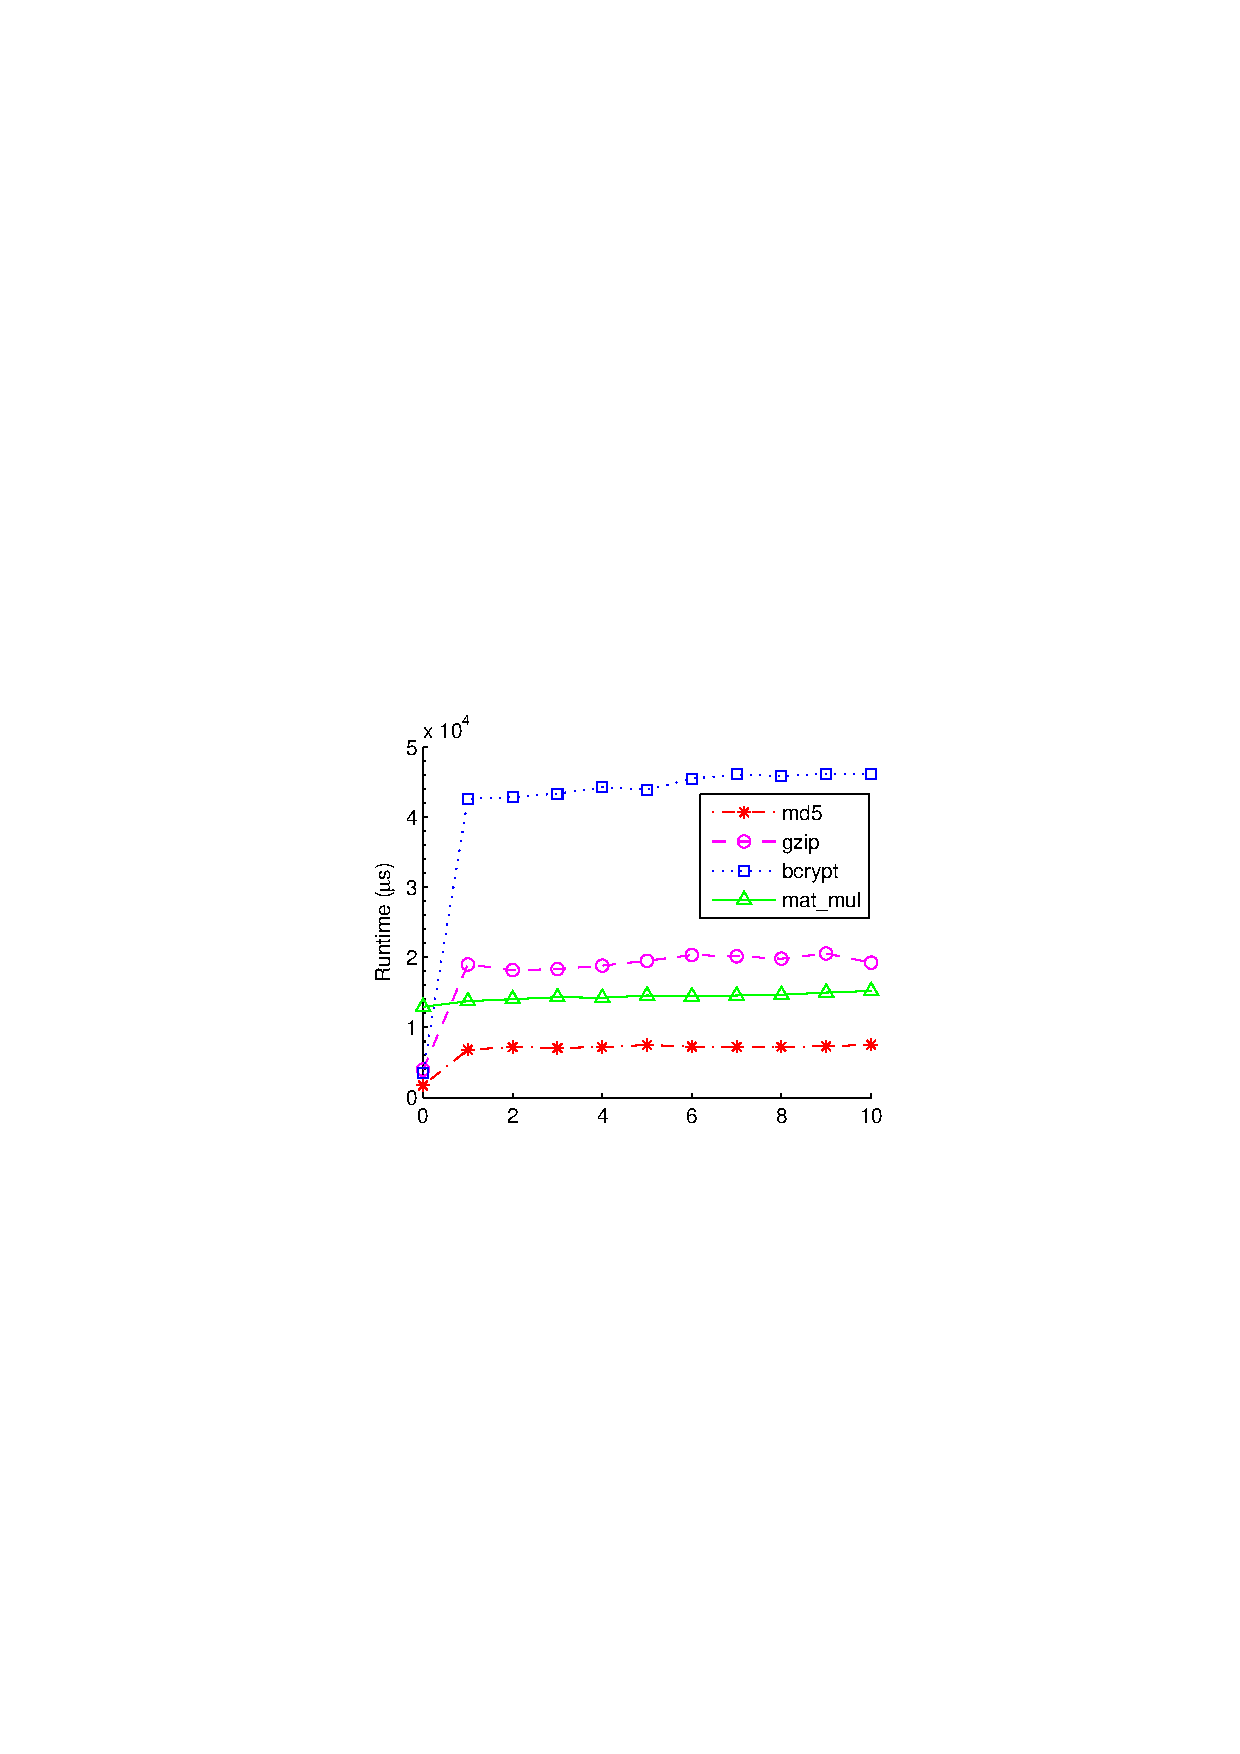
\includegraphics[width=0.9\textwidth]{fig/runtime.pdf}
\caption{The impact on runtime performance ($\mu$s) of DCVP with different partitions.}
\label{fig:runtime}
%\end{figure}
\end{minipage}

\begin{minipage}[t]{0.48\textwidth}
%\begin{figure}[t]
\centering
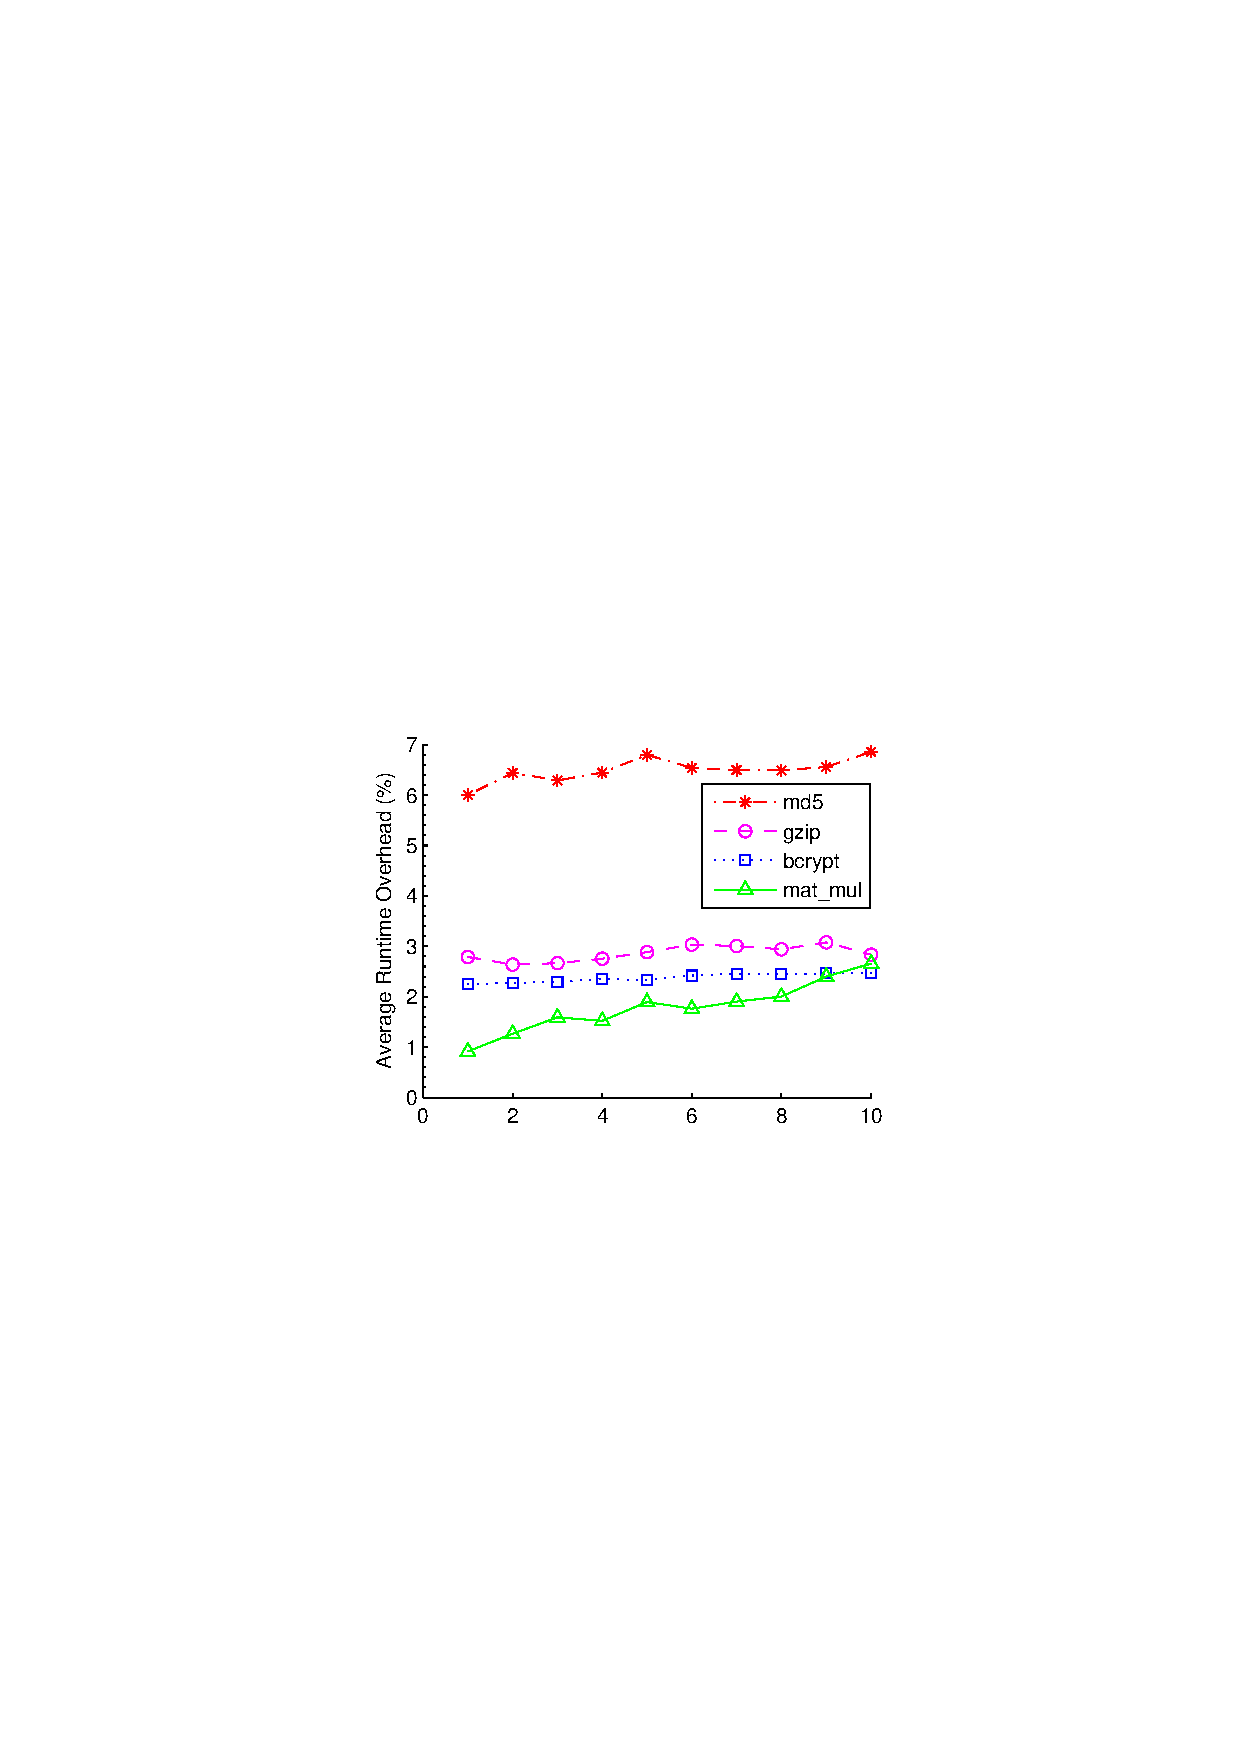
\includegraphics[width=0.9\textwidth]{fig/avg_runtime.pdf}
\caption{The average runtime overhead per dynamically executed critical instruction.}
\label{fig:avgruntime}
%\end{figure}
\end{minipage}
\begin{minipage}[t]{0.48\textwidth}
%\begin{figure}[t]
\centering
\includegraphics[width=0.9\textwidth]{fig/opfreq.pdf}
\caption{The average frequencies of \textit{opcodes}. The horizontal axis specifies the \textit{opcodes}.}
\label{fig:freq}
%\end{figure}
\end{minipage}

\begin{minipage}[t]{0.48\textwidth}
%\begin{figure}[t]
\centering
\includegraphics[width=0.9\textwidth]{fig/figfilecom.pdf}
\caption{The comparison of impact on file size (KB) with VMProtect and Themida.}
\label{fig:filecom}
%\end{figure}
\end{minipage}
\begin{minipage}[t]{0.48\textwidth}
%\begin{figure}[t]
\centering
\includegraphics[width=0.9\textwidth]{fig/figtimecom.pdf}
\caption{ The comparison of runtime performance ($\mu$s) with VMProtect and Themida.}
\label{fig:timecom}
\end{minipage}
\end{figure*}



To evaluate the runtime overhead that DCVP introduces, we run the obfuscated programs for several times and calculate the average execution time of them: \texttt{md5}, \texttt{gzip}, and \texttt{bcrypt} are used to process a text file (\texttt{test.txt}) of 10KB; \texttt{matrix\underline{ }mul} is used to calculate the product of two 5$\times$5 matrices. The average execution time is shown in figure \ref{fig:runtime}. Among them, \texttt{bcrypt} has the largest increase of execution time from original program\footnote{The execution time of the original program is specified by ``\texttt{0}" on the horizontal axis.} to the obfuscated program with one partition. This resulted from that the critical instructions in \texttt{bcrypt} is executed much more times than others (as shown in the last column in table \ref{tab:statistics}). Besides, the execution time changes little as the number of partitions increases. From section~\ref{sec:partition-random} we can learn that if the number of partitions increases by one, the program only needs to execute an extra \texttt{handler} to interpret the \texttt{switch\underline{ }HAT} instruction. The introduced runtime overhead is negligible. In some situations, the execution time of an obfuscated program with more partitions may have a slightly lower runtime overhead. This probably results from the locality of reference \cite{locality}.



We evaluate the average runtime overhead per dynamically executed instruction. We use $T_{ob}$ to denote the execution time of a obfuscated program, $T_{o}$ for that of the original program, and $C_{e}$ for the count of the critical instructions been dynamically executed. The average runtime overhead per dynamically executed instruction is calculated by
%\[\frac{T_{ob} - T_{o}}{C_{e}}.\]
\[(T_{ob} - T_{o})/C_{e}. \]
The results are shown in figure \ref{fig:avgruntime}. From figure \ref{fig:avgruntime}, we can learn that \texttt{md5} has the largest average runtime overhead per dynamically executed instruction. The reason is that the critical code of \texttt{md5} is full of arithmetical and logical instructions, which takes a longer time to interpret.



We also put the four target programs together and count the average frequencies of \textit{opcodes}. We take the obfuscated programs with 1, 2, 4, 8, 16, and 32 partitions for comparison. The results are presented in figure \ref{fig:freq}. As we can see, as the number of partitions increases, the frequencies of \textit{opcodes} tend to be closer.

Finally, we use two commercial code virtualization protection system for comparison, VMProtect~\cite{vmp} and Themida~\cite{Themida}. Figure~\ref{fig:filecom} shows the impact of the three virtualization protection system on the file size of the four target programs. The cost of Themida is much greater than the other two system, and the impact of DCVP and VMProtect is similar. This result should be related to the design of virtual instructions and \texttt{handlers}. Runtime overhead as shown in Figure~\ref{fig:timecom}. In general, the effects of the three protection systems are similar. Special, the runtime overhead of \texttt{bcrypt} that protected by Themida is far greater than the other target programs.




\section{Related Work}
Software protection is used to protect the intellectual property encapsulated within software programs from been understood and modified, by transforming target program into a more obscure and hard-understanding one. The earliest published works in software protection can be traced back to 1980, Kent \cite{kent1981protecting} addressed the security requirements of software vendors: protection from software copying and modification. During the past decades, numerous approaches of software protection have been proposed, e.g. junk instructions, equivalent instructions \cite{nicolaou2009applied}, code encryption, control flow and data flow obfuscation \cite{collberg2002watermarking,liem2008compiler,ge2005control}, etc. These approaches alone provide only limited obscurity, and one protection system usually integrates several of these and makes them work together to provide a certain level of obscurity.


In recent years, there have been many code protection technology and their focus is different. Such as, control flow integrity~\cite{Zhang2013Practical,Zhang2013Control} provide a strong protection against modern control flow hijacking attacks, including those based on Return-Oriented Programming (ROP). Code Randomization, Stephen Crane et al.~\cite{Crane2015Readactor} presents a practical, fine-grained code randomization defense, called Readactor, resilient to both static and dynamic ROP attacks. At the same time, the code reverse analysis technology is developing. Symbolic and concolic execution~\cite{Yadegari2015Symbolic} and Data flow tracking and tanit analysis~\cite{Jee2012A,Balliu2014Automating,Yadegari2015A} can find important applications in a number of security-related program analyses, including analysis of malicious code. This paper focuses on the code virtualization protection and its reverse analysis technology.


Code virtualized obfuscation, aka VM-based obfuscation, has recently been used to protect software from malicious reverse engineering \cite{cv,vmp,fang2011multi,wang2014tdvmp,wang2013nislvmp}. In Section 2 we have already introduced the details of VM-based obfuscation and possible attacks. Existing researches on VM-based obfuscation focus on foiling reverse analysis. TDVMP \cite{wang2014tdvmp} obfuscates \texttt{handlers} to generate multiple semantics-equivalent but appearance-different ones and embeds them into target program. At runtime, it will execute different instructions since the execution of each \texttt{handler} is chose from the several candidates randomly, i.e., the obfuscated program has a per-process execution diversity. This is especially useful for defeating dynamic analysis. Fang et al. \cite{fang2011multi} presented a multi-stage obfuscation method that iteratively transforms a program for many times in using different interpretations. DCVP focuses on invalidating the analysis knowledge about the semantics of bytecode instructions and preventing from quick and large scale reverse analyses, which is orthogonal to the above approaches and is complementary to them.

DCVP adopts ISR (Instruction Set Randomization) techniques while generating randomized and distinct virtual instruction sets. ISR has been used to prevent code injection attacks by randomizing the underlying system instructions \cite{barrantes2003randomized,kc2003countering,portokalidis2010fast}. In this approach, instructions are encrypted with a set of random keys and then decrypted before being fetched and executed by the CPU. ISR is effective for defeating code injection attacks but cannot prevent from reverse engineering attacks. As in our attack model, software programs are executed in a malicious host environment, where attackers are able to trace and log the decrypted instructions for later analysis. DCVP employs an approach similar to ISR while generating random virtual instruction sets, by changing the relationship between the opcodes and the virtual instructions \cite{kc2003countering}, but it never ``decrypts" the virtual instructions back into their original ones. Instead, DCVP uses \texttt{handlers} to interpret the virtual instructions. Since \texttt{handlers} of virtual instructions are more complex than their corresponding native instructions, DCVP can prevent software programs from been reverse engineered easily. Besides, DCVP uses different ISRs in a single program, making the reverse analyses even more difficult and tedious.



\section{Conclusion}
In this paper, we have introduced the internals of code virtualized obfuscation and the process of reverse analyzing a VM-obfuscated program. Although such obfuscation poses a great obstacle to an analyst, the presence of \textit{analysis knowlege} can ease the work of an analyst work. To mitigate the effect of reuse of \textit{analysis knowlege}, we present DCVP, which disables the \textit{analysis knowlege} by randomizing the semantics of bytecode instructions. Furthermore, DCVP partitions the generated virtual instructions into several parts, each been encoded differently. This defeats the attempts to infer the semantics of bytecode instructions based on the non-uniform frequencies of \textit{opcodes}. Our evaluations show that DCVP is effective for mitigating the effect of reuse of \textit{analysis knowlege}. As future work, we plan to: (1) use existing virtual instructions to switch the HAT instead of the specific \texttt{switch\underline{ }HAT} for sake of the stealthiness of the switching; %(2) obfuscate \texttt{handlers} differently for different partitions;
(2) work on data flow obfuscation to defeat semantics-based de-obfuscation.




% conference papers do not normally have an appendix


% use section* for acknowledgement
%\section*{Acknowledgment}
%This work was supported in part by the National Natural Science Foundation of China (No. 61373177, and No. 61572402), the Key Project of Chinese Ministry of Education (No. 211181), the International Cooperation Foundation of Shaanxi Province, China ((No. 2013KW01-02, No. 2015KW-003 and No. 2016KW-034), the China Postdoctoral Science Foundation (grant No. 2012M521797), the Research Project of Shaanxi Province Department of Education (No. 15JK1734), and the Research Project of NWU, China (No. 14NW28).





% trigger a \newpage just before the given reference
% number - used to balance the columns on the last page
% adjust value as needed - may need to be readjusted if
% the document is modified later
%\IEEEtriggeratref{8}
% The "triggered" command can be changed if desired:
%\IEEEtriggercmd{\enlargethispage{-5in}}

% references section

% can use a bibliography generated by BibTeX as a .bbl file
% BibTeX documentation can be easily obtained at:
% http://www.ctan.org/tex-archive/biblio/bibtex/contrib/doc/
% The IEEEtran BibTeX style support page is at:
% http://www.michaelshell.org/tex/ieeetran/bibtex/
%\bibliographystyle{IEEEtranS}
% argument is your BibTeX string definitions and bibliography database(s)
%\bibliography{IEEEabrv,../bib/paper}
%
% <OR> manually copy in the resultant .bbl file
% set second argument of \begin to the number of references
% (used to reserve space for the reference number labels box)

\bibliographystyle{IEEEtran}
\bibliography{randvmp_bib}

%\begin{thebibliography}{1}

%\bibitem{IEEEhowto:kopka}
%H.~Kopka and P.~W. Daly, \emph{A Guide to \LaTeX}, 3rd~ed.\hskip 1em plus
 % 0.5em minus 0.4em\relax Harlow, England: Addison-Wesley, 1999.

%\end{thebibliography}




% that's all folks
\end{document}


